\chapter{Investigating Urban Soundscapes of the COVID-19 Lockdown: A predictive soundscape modelling approach}
\label{ch:lockdown}
\markright{\cref{ch:lockdown}. Soundscapes of the COVID-19 Lockdown: A predictive modelling approach}

The engineering soundscape approach developed in this thesis strives to make certain applications of soundscape possible. As highlighted earlier, one of these applications is the ability to assess the soundscape perception in situations where surveys are impractical as well as to be able to track changes in the soundscape of public spaces. This chapter therefore presents a unique application of predictive modelling towards these goals as well as the development of the predictive modelling method itself. First, I will review the identified impacts of the \gls{covid19} lockdowns on the sound environment in cities around the world, investigate these changes in detail within London and Venice, and finally presents the impact of these changes on the likely perception of the soundscape of public spaces through the results of the predictive model. 

%%%%%%%%%%%%%%%%%%%%%%%%%%%%%%%%%%%%%%%%%%%%%%%%%%%%%%%%%%%%%%%%%%%%%%%%

\section{Review of the impacts of COVID-19}
 \label{sec:covidReview}
 The global emergency caused by \gls{covid19} in early 2020 required national lockdown measures across the world, primarily targeting human activity. In the United Kingdom, construction and transport were allowed to continue, but a decrease in activity was observed \citep{Hadjidemetriou2020impact}. During some periods and in other countries, such as Italy, the restrictions were more severe and even included limiting people's movement to a certain radius from their place of residence \citep{Ren2020Pandemic}. Explorations in environmental acoustics of lockdown conditions across the world have revealed various degrees of impact on the acoustic environment, with researchers reporting reductions in noise levels affecting the population at the scale of urban agglomerations such as the Ruhr Area in Germany \citep{Hornberg2021Impact} and conurbations in the south of France \citep{Munoz2020Lockdown}. Impacts have also been reported at a scale of a multimillion city such as Madrid \citep{Asensio2020Changes} or Barcelona \citep{BonetSola2021Soundscape} as well as at a more local, city-centre or even public space-scale in cities such as Stockholm \citep{Rumpler2021Noise}, London \citep{Aletta2020Assessing}, Girona \citep{AlsinaPages2021Changes}, or Granada \citep{VidaManzano2021sound}. In general, these studies have demonstrated a decrease in urban noise levels, indicating a difference in the amount of decrease depending on the type of space investigated (e.g. parks, urban squares, etc.) and the type of human activity characteristic for the space, with higher reductions in places typically associated with human sounds and activities such as shopping and tourism.

 \subsection{The lockdown measures in London and Venice}

In general, the lockdown measures implemented in the UK to contain the spread of the SARS-CoV-2 virus involved `stay at home' recommendations, social distancing, stopping non-essential commercial activities, banning public gatherings, limiting traffic mobility, etc. Specifically, the UK Government passed the Health Protection (Coronavirus, Restrictions) (England) Regulations 2020, which were put into place at 1:00 pm on \nth{26} March 2020 \citep{PHE2020Health}. Under these restrictions, the public were only allowed to leave their homes once per day for essential activities and exercise. All offices and shops selling non-essential goods were told to close, gatherings of more than two people in public were banned, and individuals were advised to only interact with members of their own household. These restrictions were set to be reviewed by the Secretary of State at least once every 21 days and would continue indefinitely until they were no longer necessary to prevent the spread of infection in England. In practice the lockdown continued through the spring of 2020 and was first partially eased on the \nth{1} of June, with school children in England returning to school, but the broader lockdown continued throughout the summer \citep{Tong2021Increases}. During this period of lockdown, noise complaints increased by 48\% compared to the same period during the preceding year, with an immediate uptick seen once lockdown measures were implemented. \cref{fig:noiseComplaints} shows the timeline of these restrictions and the accompanying noise complaints received by 22 boroughs in London \citep{Tong2021Increases}.

\begin{figure}[h]
  \centering
  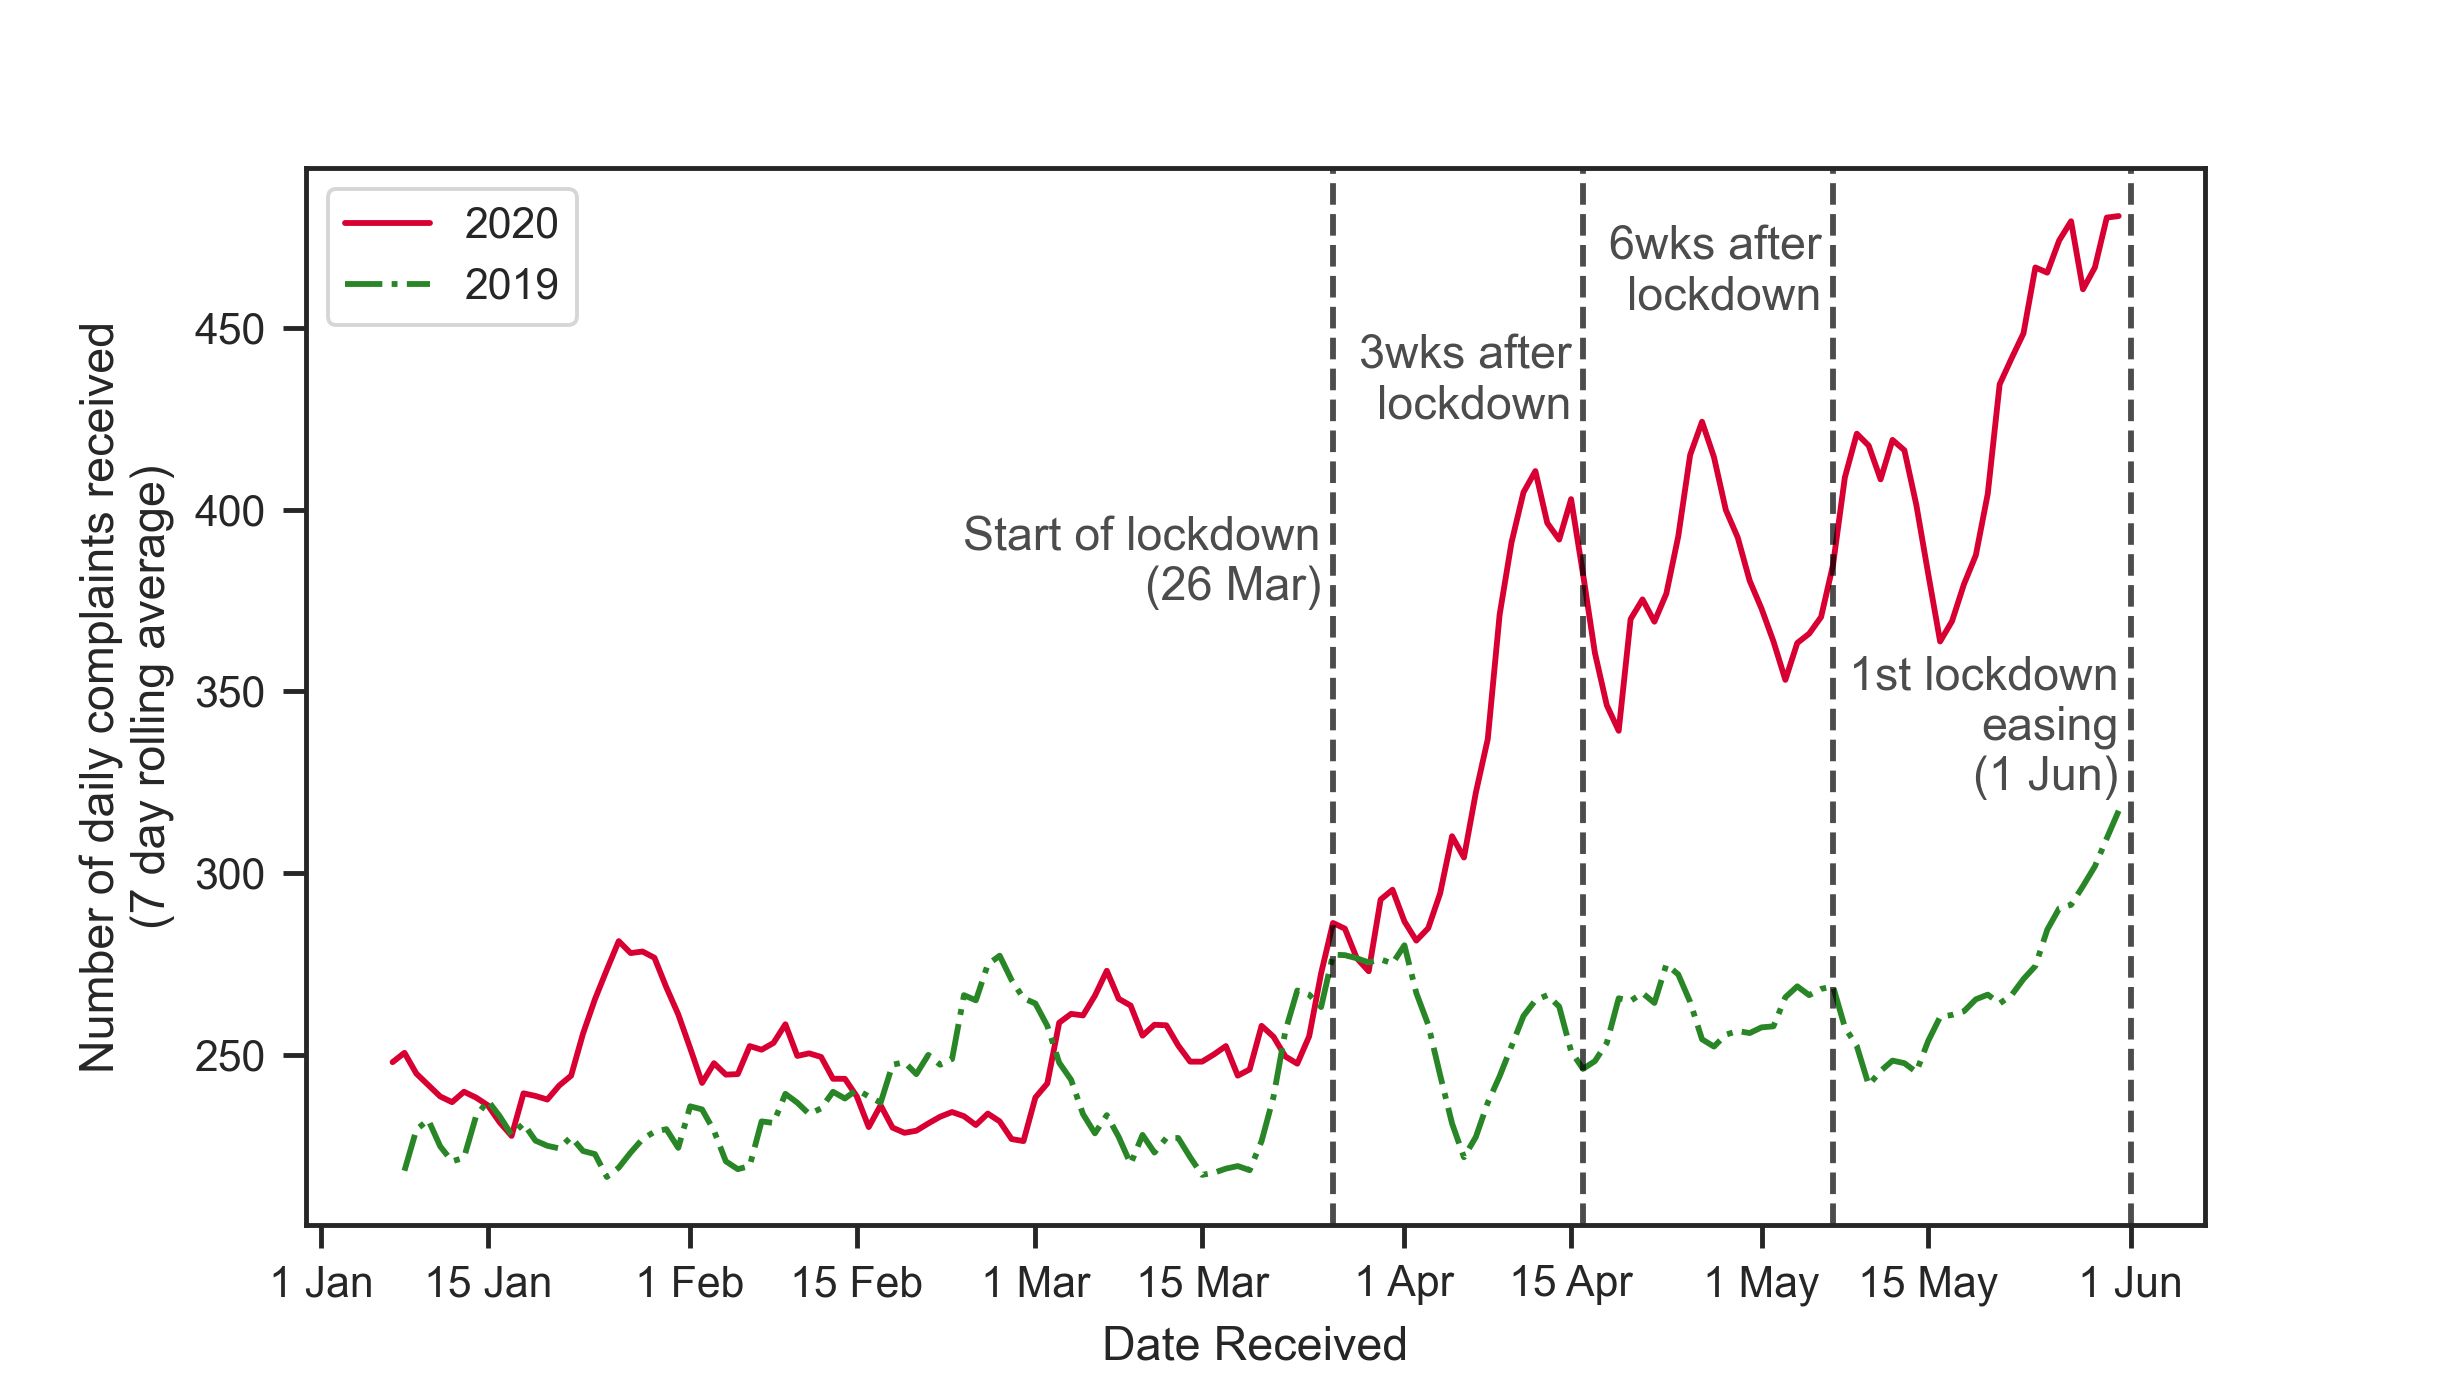
\includegraphics[width=\textwidth]{Figures/LockdownNoiseComplaints-TimeSeriesPlot_3.png}
  \caption[Time series of the number of noise complaints received in the first half year of 2019 and 2020. A 7-day rolling average window is applied to account for weekly patterns in noise complaint reporting.]{Time series of the number of noise complaints received in the first half year of 2019 and 2020 for 22 boroughs in London. A 7-day rolling average window is applied to account for weekly patterns in noise complaint reporting\footnotemark. \label{fig:noiseComplaints}}
\end{figure}

\footnotetext{Figure originally created for \citet{Tong2021Increases}.}

\subsection{Perceptual changes}

 Those studies were mostly focussed around the \gls{laeq}, as well as a standardization approach to reporting subsequent changes in soundscape proposed by \citet{Asensio2020Taxonomy}. They were not able to reveal the perceptual impact of such conditions in public spaces as well because of: 1) the lack of subjective data for the exact or comparable locations in previous years; and 2) the lack of participants present in public spaces during the lockdown, hence the inability to collect soundscape data \emph{in-situ}. Attempts have been made to bridge this gap by using social networks to source subjective data, but this resulted in a focus on indoor conditions following the shift in the citizens' behaviour, i.e. spending more time indoors \citep{Bartalucci2021survey,Lee2021Attitudes}. \citet{GarridoCumbrera2021Perceptions} relied on an online survey deployed in England, Ireland, and Spain to explore the perceived change in natural environments in particular. They observed a consistent increase in the perceived presence of natural sounds across all major cities and rural areas respectively in these three countries. A very similar trend was observed in Argentina, also based on an online questionnaire without a listening task \citep{Maggi2021Perception}. 
 
 \citet{Munoz2020Lockdown} combined noise measurements with an online questionnaire deployed to residents, some of which were residing in the areas covered by the noise monitoring network available. The participants were asked to recall how their lockdown area sounded before and during the first lockdown in 2020 and to describe the perceived change. They observed a consistent reduction in levels, followed by the perceived reduction of transport sounds (air and road) and an increase of natural sounds, while the resulting environment was described as pleasant, calm, and peaceful. By combining field recordings and focus groups, \citet{Sakagami2020How} and \citet{Lenzi2021Soundscape} observed changes in the sound source composition and the affective quality of soundscape in a residential area in Kobe, Japan and a public space in Getxa, Spain, respectively, during the different stages of the lockdown period. Following the easing of lockdown measures, a decrease in animal and traffic sounds was observed in Kobe, while an increase in eventfulness, loudness, and presence of human sound sources, followed by a decrease in pleasantness, was shown in Getxa.

 This metric- and , by necessity, indoor-focussed approach left the following research questions unanswered:

\begin{enumerate}
  \item How would people have perceived these outdoor urban spaces as a result of this change in acoustic environment? (RQ1)
  \item Would these sound level reductions result in improvements to the soundscape of the spaces? (RQ2)
  \item What are the key features needed for a soundscape prediction model based on comprehensive acoustic on site measurements to be used for assessing locations with low social presence or in situations where conducting surveys is impractical (RQ3)?
\end{enumerate}

The \nth{1} research question (RQ1), addressing the perceptual effect of the change in urban soundscape induced by the lockdowns, can be further broken down into the following questions:

\begin{itemize}
  \item How was the sound source composition influenced by the change?
  \item How would the affective response to the acoustic environment in lockdowns change?
  \item Could this demonstrate the effect of human activities on the perception of an acoustic environment in general?
\end{itemize}

%%%%%%%%%%%%%%%%%%%%%%%%%%%%%%%%%%%%%%%%%%%%%%%%%%%%%%%%%%%%%%%%%%%%%%%%

\section{Materials and methods}

 This study was conducted via initial onsite data collection campaigns in Central London and Venice in 2019 before the outbreak of \gls{covid19} as part of the \gls{ssid} project \citep{Mitchell2020Soundscape} and in 2020 during the strictest part of the lockdowns \citep{Aletta2020Assessing}, including objective acoustic data (2019 and 2020) and subjective responses (2019 only). 
 
 Using both 2019 and 2020 binaural recordings, an online listening experiment was conducted to provide an understanding about the change in sound source composition. The 2019 onsite questionnaire data were used to define the dominant sound source at each location as a starting point for interpreting the soundscape change. A predictive model was developed to reveal the change in the perceived pleasantness and eventfulness using objective acoustic data and location to predict subjective responses. Although the initial (2019) dataset contains additional locations (specifically, in Spain, the Netherlands, and China), due to the nature of this study as a reaction to the strict movement and activity restrictions, the sites which could be included in the lockdown (2020) measurement campaigns were limited to locations where staff and equipment had access and where recordings could be undertaken during the spring of 2020.

 The sites were selected to provide a mixture of sizes and uses, varying in typology ranging from paved squares to small and large parks to waterside spaces across both cities. Throughout the text they are indexed via a LocationID based on the location's name (e.g. CamdenTown, SanMarco), while a more in-depth overview of each is given in \cref{app:location-data}. London is taken as an example of a large, typically noisy city while the Venice sample provides a unique look at spaces with typically very high human activity levels and no road traffic activity. In particular, the 2019 Venice surveys were taken to coincide with the yearly Carnevale festival in order to capture its distinct soundscape.

\citet{ISO12913Part2} was consulted for reporting on soundscape data. A detailed description of the 2019 survey campaigns is featured through the paper and in the public database. This study was approved by departmental UCL IEDE Ethics Committee on \nth{17} July 2018 for onsite data collection and on the \nth{2} of June 2020 for the online listening experiment and is conducted in adherence to the ethical requirements of the Declaration of Helsinki \citep{WMA2013World}.

 \subsection{Onsite data: Questionnaires, binaural measurements, and recordings}
  The 2019 data collection was performed across all the locations using the protocol based on the Method A of the ISO/TS 12913-2:2018 \citep{ISO12913Part2}, collected either via handheld tablets or paper copies of the questionnaire. The full questionnaire and data collection procedure are given in \cref{app:questionnaire} and \cref{chap:protocol}, respectively, however the key parts used for this study are those addressing sound source dominance and \gls{paq}.
   
   The initial onsite data collection featured both questionnaire data collected from the general public and acoustic measurements, conducted across thirteen urban locations (in London $N=11$, in Venice $N=2$) between the \nth{28} of February and the \nth{21} of June 2019, with additional sessions in July and October 2019. Although the total survey period in 2019 extended over several seasons, the surveys at any individual location did not extend over seasons with different occupancy patterns. A total of 1,318 questionnaire responses were collected from the general population across the measurement points during 1 -- 3 hour-long campaigns in both cities in 2019, accompanied by 693 approximately 30-second long 24-bit 44.1 kHz binaural recordings. After data cleaning, each of the 13 locations was characterised by between 14 to 80 recordings and between 24 to 147 questionnaire responses. Mean age of the participants was 33.9, with a standard deviation of 14.57 (45\% male, 53.8\% female, 0.4\% non-conforming, 0.9\% prefer-not-to-say). Psychoacoustic analyses of the binaural recordings were performed as described in \cref{sec:analyses}.

   Although recent results from both \citet{Tarlao2020Investigating} and \citet{Erfanian2021Psychological} indicate the important influence of personal and demographic factors -- in particular age and gender -- on soundscape perception, these factors were not included as potential features in the modelling process\footnote{See \cref{ch:whostudy} for the results of \citet{Erfanian2021Psychological} and an in depth discussion of how these factors could or should be integrated into the predictive modelling process.}. Given the nature of this study as addressing a scenario when people could not be surveyed, no additional demographic information is available in the lockdown case to be fed into the model and is therefore not useful to include for the development and application of this specific predictive model. This information is reported throughout the study simply to provide further context to the data collection.

   The subsequent measurement campaign in 2020 mimicked the binaural recording strategy applied in the initial campaign and was performed between the \nth{6} and the \nth{25} of April 2020 in both cities, this time excluding the questionnaire. An additional 571 binaural recordings were collected on site in 2020.


\begin{sidewaystable}[hp]
\centering
\caption{Pearson correlation coefficients between candidate acoustic features and ISOPleasant and ISOEventful across all 13 locations. Only statistically significant ($p < 0.01$) coefficients are shown. \label{tab:corr}}
\begin{tabular}{r|cccccccccccc} 
\toprule
\textbf{Parameter} & ISOPl & ISOEv & $PA$ & $N_5$ & $S$ & $R$ & $I$ & $FS$ & $T$ & $L_{Aeq}$ & $L_{A10}-L_{A90}$ & $L_{Ceq}-L_{Aeq}$ \\ 
\midrule
ISOPleasant &  &  &  &  &  &  &  &  &  &  &  &  \\
ISOEventful & -0.24 &  &  &  &  &  &  &  &  &  &  &  \\
$PA$ & -0.28 & 0.24 &  &  &  &  &  &  &  &  &  &  \\
$N_5$ & -0.37 & 0.33 & 0.94 &  &  &  &  &  &  &  &  &  \\
$S$ &  &  & 0.71 & 0.56 &  &  &  &  &  &  &  &  \\
$R$ & -0.36 & 0.32 & 0.63 & 0.74 & 0.11 &  &  &  &  &  &  &  \\
$I$ &  &  & -0.10 &  & -0.37 & 0.24 &  &  &  &  &  &  \\
$FS$ & -0.11 & 0.14 & 0.37 & 0.43 &  & 0.46 & 0.55 &  &  &  &  &  \\
$T$ & -0.21 & 0.30 & 0.58 & 0.63 & 0.12 & 0.54 & 0.16 & 0.52 &  &  &  &  \\
$L_{Aeq}$ & -0.34 & 0.37 & 0.84 & 0.93 & 0.56 & 0.72 & -0.09 & 0.37 & 0.57 &  &  &  \\
$L_{A10}-L_{A90}$ & -0.18 & 0.15 & 0.21 & 0.33 & -0.20 & 0.31 & 0.36 & 0.44 & 0.40 & 0.23 &  &  \\
$L_{Ceq}-L_{Aeq}$ &  & -0.20 & -0.49 & -0.49 & -0.54 & -0.31 &  & -0.27 & -0.28 & -0.61 & -0.22 &  \\
$RA$ & -0.34 & 0.31 & 0.60 & 0.74 & 0.18 & 0.71 & 0.31 & 0.63 & 0.58 & 0.73 & 0.23 & -0.14 \\
\bottomrule
\end{tabular}
\end{sidewaystable}

   \cref{tab:corr} shows the Pearson correlation coefficient between each of the candidate acoustic features and the outcome pleasantness and eventfulness. As all variables considered are continuous, and the eventual model is linear, the Pearson coefficient is chosen as a measure of the strength of the linear relationship between two continuous variables. For \gls{isopl} ($ISOPl$), we can see three tiers of correlations:

   \begin{enumerate}
     \item The more highly correlated tier ($|r| > 0.28$) consists of \gls{ra}, \gls{laeq}, \gls{r}, \gls{n5}, and \gls{pa}
     \item The low correlation tier consists of \gls{la10la90}, \gls{tu}, and \gls{iu}
     \item \gls{lcla}, \gls{iu}, and \gls{s} show no correlation
   \end{enumerate}

   For \gls{isoev} ($ISOEv$), these tiers are:
   \begin{enumerate}
     \item The more highly correlated tier ($|r| > 0.30$) consists of \gls{ra}, \gls{laeq}, \gls{tu}, \gls{r}, and \gls{n5}
     \item The low correlation tier consists of \gls{lcla}, \gls{la10la90}, \gls{fs}, and \gls{pa}
     \item \gls{iu} and \gls{s} show no correlation
   \end{enumerate}

   Among the inter-correlations for the psychoacoustic metrics considered for inclusion as input features, we can see several very highly correlated features (i.e. $>0.9$). As expected, \gls{pa}, \gls{laeq}, and \gls{n5} are highly correlated, meaning that careful consideration is paid to these features to ensure they do not contribute to multicollinearity in the final model.

%%%%%%%%%%%%%%%%%%%%%%%%%%%%%%%%%%%%%%%%%%%%%%%%%%%%%%%%%%%%%%%%%%%%%%%%

   \begin{figure}[h]
     \centering
     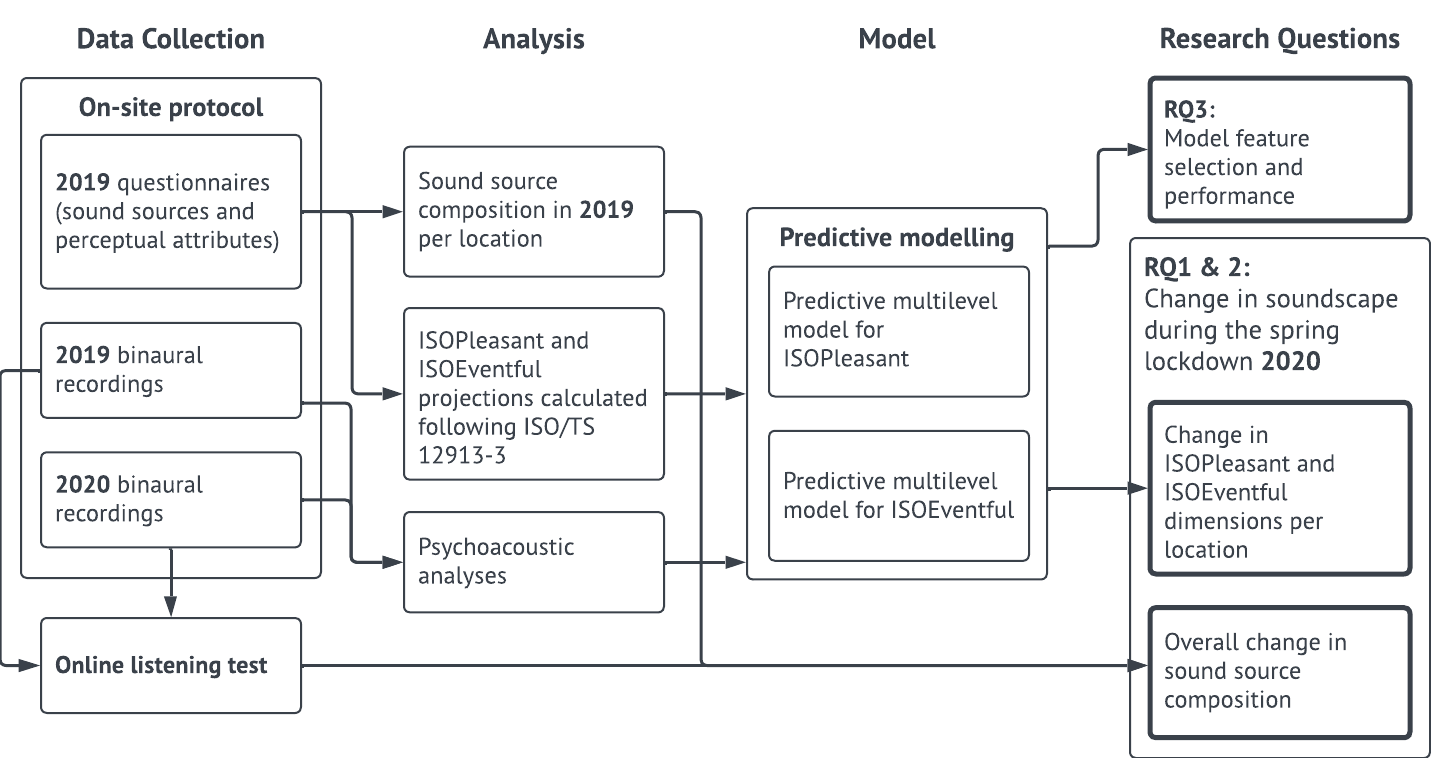
\includegraphics[width=\textwidth]{Figures/Lockdown-Fig1.png}
     \caption{The study flowchart indicating the data collection, analysis, modelling, and discussion throughout the study. \label{fig:lockdown-study-framework}}
   \end{figure}

%%%%%%%%%%%%%%%%%%%%%%%%%%%%%%%%%%%%%%%%%%%%%%%%%%%%%%%%%%%%%%%%%%%%%%%%

 \subsection{Modelling}

   Two linear multi-level models (MLM) were computed to predict: 1) \gls{isopl}, and 2) \gls{isoev}. These models are trained on the 2019 data only, then applied to the acoustic data collected during the 2020 lockdowns, the results of which are reported in \cref{sec:applicationLockdown}. The individual-level of the models is made up of the acoustic features calculated from the binaural recordings made during each respondent's survey period, while the group-level includes the categorical `LocationID' variable indicating the location in which the survey was taken, acting as a non-auditory contextual factor. The performance criterion used for the feature selection process was the \gls{aic} \citep{Akaike1974new}.

   All of the input features are numeric values, in the units described above. Before conducting feature selection, the input features are z-scaled to enable proper comparison of their effect sizes. After the feature selection, the scaled coefficients are used in the text when reporting the final fitted models to facilitate discussion and comparison between the features. The unscaled model coefficients are reported in \cref{app:lockdown} to enable the models to be applied to new data. In order to properly assess the predictive performance of the model, an 80/20 train-test split with a balanced shuffle across LocationIDs was used. The z-scaling and feature selection were performed on the training set only, in order to prevent data leakage. To score the performance of the model on the training and testing sets, I use the \gls{mae}, which is in the scale of the response feature -- for \gls{isopl} and \gls{isoev} this means our response can range from $-1$ to $+1$. However, since the end-goal of the model is to predict the soundscape assessment of the location as a whole, rather than the individual responses, I also assess the performance of the model in predicting the average response in each location. To do this, the mean response value for each location is calculated, and the $R^2$ accuracy across LocationIDs is reported for both the training and testing sets.

   The model fitting and feature selection was performed using the \texttt{step} function from \texttt{lmerTest} (v3.1.3) \citep{Kuznetsova2017lmerTest} in R statistical software (v.4.0.3) \citep{RCT2018R}. The summaries and plots were created using the \texttt{sjPlot} package (v.2.8.6) \citep{Luedecke2021sjPlot} and \texttt{seaborn} (v.0.11.1) \citep{Waskom2021seaborn}.

 \subsection{Online survey}
\label{sec:GorillaTin}
 
   A online listening test was conducted using the Gorilla Experiment Builder\footnote{The development of this online survey was performed by Ms. Magdalena Kachlicka and Dr. Tin Oberman and the text of \cref{sec:GorillaTin} was originally drafted by Dr. Oberman. The text is included here verbatim from \citet{Mitchell2021Investigating} to accurately reflect the methods used and provide context for the later discussions.} \citep{AnwylIrvine2019Gorilla}. The participants were exposed to a random selection of 78 binaural recordings (39 from 2019 and 39 from 2020, 6 recordings per location). Each participant had the option to evaluate either 1 or 2 sets of 6 recordings randomly assigned between 13 stimuli sets. Mp3 files, converted at 256 kBps were used due to the requirements of the Gorilla platform.

%%%%%%%%%%%%%%%%%%%%%%%%%%%%%%%%%%%%%%%%%%%%%%%%%%%%%%%%%%%%%%%%%%%%%%%%

\begin{sidewaystable}
\centering
\caption{Mean and standard deviation values for 2019 and 2020 (Lockdown) measurement campaigns. The difference is the 2020 mean value subtracted from the 2019 mean value to demonstrate the level of change due to the lockdown. \emph{p}-values calculated for one-tailed t-test. }
\label{tab:LockdownNumbers}
\resizebox{\linewidth}{!}{%
\begin{tabular}{cc|cccc|cccc|ccc} 
\toprule
~ & ~ & \multicolumn{4}{c|}{\textbf{2019 }} & \multicolumn{4}{c|}{\textbf{2020 (Lockdown) }} & \multicolumn{3}{c}{\textbf{Difference and t test p-value }} \\
\textbf{LocationID} &  & \textbf{Samples} & \textbf{N5 (sone)} & \textbf{S (acum)} & $L_{Aeq}$ (dB) & \textbf{Samples} & \textbf{N5 (sone)} & \textbf{S (acum)} & $L_{Aeq}$ (dB) & \textbf{N5 (sone)} & \textbf{S (acum)} & $L_{Aeq}$ (dB) \\ 
\hline
CAM & Mean & \multirow{2}{*}{90 ~} & 39.29 & 2.28 & 72.41 & \multirow{2}{*}{44 ~} & 30.50 & 1.87 & 67.19 & -8.79** & -0.41** & -5.21** \\
 & Std. Deviation &  & 13.74 & 0.47 & 5.08 &  & 8.43 & 0.17 & 3.72 & 0.00 & 0.00 & 0.00 \\
EUS & Mean & \multirow{2}{*}{99 ~} & 31.16 & 2.25 & 69.55 & \multirow{2}{*}{38 ~} & 24.72 & 1.88 & 66.03 & -6.44** & -0.38** & -3.52** \\
 & Std. Deviation &  & 5.62 & 0.13 & 2.76 &  & 7.34 & 0.21 & 4.25 & 0.00 & 0.00 & 0.00 \\
MAR & Mean & \multirow{2}{*}{92 ~} & 12.83 & 1.67 & 55.85 & \multirow{2}{*}{41 ~} & 9.34 & 1.53 & 51.27 & -3.48** & -0.15** & -4.58** \\
 & Std. Deviation &  & 3.15 & 0.15 & 2.66 &  & 2.62 & 0.23 & 2.86 & 0.00 & 0.01 & 0.00 \\
PAN & Mean & \multirow{2}{*}{78 ~} & 15.32 & 1.64 & 59.42 & \multirow{2}{*}{80 ~} & 14.97 & 2.04 & 58.11 & -0.35 & 0.40** & -1.30** \\
 & Std. Deviation &  & 2.28 & 0.11 & 1.82 &  & 6.80 & 0.51 & 6.06 & 0.36 & 0.00 & 0.06 \\
RPF & Mean & \multirow{2}{*}{107 ~} & 11.98 & 1.67 & 54.47 & \multirow{2}{*}{43 ~} & 8.18 & 1.40 & 49.61 & -3.79* & -0.28** & -4.86** \\
 & Std. Deviation &  & 7.31 & 0.17 & 5.01 &  & 2.19 & 0.16 & 2.76 & 0.04 & 0.00 & 0.00 \\
RPJ & Mean & \multirow{2}{*}{82 ~} & 16.90 & 2.72 & 59.72 & \multirow{2}{*}{35 ~} & 15.38 & 2.64 & 58.45 & -1.52 & -0.08 & -1.27 \\
 & Std. Deviation &  & 8.20 & 0.65 & 8.21 &  & 7.15 & 0.59 & 7.35 & 0.26 & 0.33 & 0.30 \\
RUS & Mean & \multirow{2}{*}{149 ~} & 23.07 & 2.62 & 65.49 & \multirow{2}{*}{40 ~} & 12.04 & 1.47 & 55.00 & -11.03** & -1.15** & -10.49** \\
 & Std. Deviation &  & 5.10 & 0.48 & 3.58 &  & 3.35 & 0.10 & 3.00 & 0.00 & 0.00 & 0.00 \\
SPC & Mean & \multirow{2}{*}{60 ~} & 18.22 & 1.81 & 62.40 & \multirow{2}{*}{27 ~} & 13.18 & 1.46 & 56.33 & -5.04** & -0.35** & -6.07** \\
 & Std. Deviation &  & 3.81 & 0.12 & 2.88 &  & 3.21 & 0.10 & 2.58 & 0.00 & 0.00 & 0.00 \\
SPR & Mean & \multirow{2}{*}{57 ~} & 19.72 & 1.73 & 64.59 & \multirow{2}{*}{48 ~} & 13.93 & 1.45 & 57.77 & -5.78** & -0.28** & -6.82** \\
 & Std. Deviation &  & 3.02 & 0.12 & 2.22 &  & 4.62 & 0.28 & 4.71 & 0.00 & 0.00 & 0.00 \\
TAT & Mean & \multirow{2}{*}{129 ~} & 19.86 & 1.76 & 63.61 & \multirow{2}{*}{41 ~} & 11.33 & 1.25 & 54.37 & -8.54** & -0.50** & -9.24** \\
 & Std. Deviation &  & 4.95 & 0.22 & 3.80 &  & 2.50 & 0.15 & 2.71 & 0.00 & 0.00 & 0.00 \\
TOR & Mean & \multirow{2}{*}{115 ~} & 22.69 & 2.03 & 64.77 & \multirow{2}{*}{41 ~} & 15.20 & 1.47 & 56.79 & -7.49** & -0.56** & -7.98** \\
 & Std. Deviation &  & 5.60 & 0.23 & 3.79 &  & 6.38 & 0.21 & 4.37 & 0.00 & 0.00 & 0.00 \\
VenMON & Mean & \multirow{2}{*}{24 ~} & 11.26 & 1.60 & 54.91 & \multirow{2}{*}{33 ~} & 8.33 & 1.70 & 51.28 & -2.93** & 0.10 & -3.63* \\
 & Std. Deviation &  & 3.54 & 0.19 & 4.84 &  & 2.71 & 0.20 & 4.46 & 0.01 & 0.06 & 0.02 \\
VenPSM & Mean & \multirow{2}{*}{90 ~} & 28.64 & 2.04 & 70.38 & \multirow{2}{*}{40 ~} & 7.09 & 1.11 & 48.36 & -21.55** & -0.92** & -22.03** \\
 & Std. Deviation &  & 7.06 & 0.18 & 4.33 &  & 2.32 & 0.12 & 3.66 & 0.00 & 0.00 & 0.00 \\ 
\hline
London & Mean & \multirow{2}{*}{1058 ~} & 21.26 & 2.05 & 63.08 & \multirow{2}{*}{478 ~} & 15.37 & 1.70 & 57.42 & -5.89** & -0.35** & -5.66** \\
~ & Std.  Deviation &  & 9.96 & 0.50 & 6.62 &  & 8.31 & 0.48 & 6.67 & 0.00 & 0.00 & 0.00 \\
Venice & Mean & \multirow{2}{*}{114 ~} & 24.98 & 1.94 & 67.13 & \multirow{2}{*}{73 ~} & 7.65 & 1.38 & 49.68 & -17.33** & -0.56** & -17.45** \\
~ & Std.  Deviation &  & 9.62 & 0.26 & 7.73 &  & 2.56 & 0.34 & 4.27 & 0.00 & 0.00 & 0.00 \\ 
\hline
Total & Mean & \multirow{2}{*}{1172 ~} & 21.62 & 2.04 & 63.47 & \multirow{2}{*}{551 ~} & 14.35 & 1.66 & 56.40 & -7.27** & -0.39** & -7.08** \\
 & Std. Deviation &  & 9.99 & 0.48 & 6.84 &  & 8.22 & 0.47 & 6.92 & 0.00 & 0.00 & 0.00 \\
\bottomrule
\end{tabular}
}
\end{sidewaystable}

   No visual stimuli were used in the experiment. The experiment consisted of:

   \begin{enumerate}
     \item an initial exercise to enhance the chances of participants complying with the instructions and wearing headphones
     \item a training set using two randomly chosen binaural recordings (then not used in the main task) from the dataset
     \item a soundscape characterisation questionnaire starting with an open-ended question about perceived sound sources and featuring the same questions as the one used in-situ, looking into the perceived affective quality of the soundscape the perceived sound source dominance of the following four types: traffic noise, other noise, human sounds, and natural sounds
     \item a questionnaire on the basic demographic factors.
   \end{enumerate}

   The questionnaire used in Part 3 of the online experiment is reported in \cref{tab:gorilla}.

   Baring in mind the remote nature of the study and to ensure a minimum level of robustness for reliable sound source recognition, an initial exercise was performed consisting of a headphone screening test \citep{Woods2017Headphone} and a headphone reproduction level adjustment test \citep{Gontier2019Estimation}. The level adjustment was performed using an 11-second-long pink noise sample matched to the lowest and the highest \gls{la90} values from the experimental set. Participants were asked to adjust their listening level to clearly hear the quieter sample while keeping the level low enough, so they don't find the louder sample disturbing. The headphone screening test followed, featuring a stereo signal of 1-second-long 100 Hz sin tone, generated with Izotope RX6 application, played at a 3 dB difference where one of the equally loud pairs had its phase inverted. A 100 Hz sin was used because the pilot tests revealed that the 200 Hz sin tone proposed by \citet{Woods2017Headphone} created a higher uncertainty varying across different laptop models and would likely contribute to the chances of a participant fooling the test. It was expected that participants using speakers would not be able to either hear the sin wave or would be fooled by the inverted phase effect and therefore not able to pass the trials, unless they were indeed using headphones. The participant needed to recognise the quietest of the 3 samples in a trial of 6 attempts. Only participants correctly answering 5 or more out of 6 trials were allowed to proceed with the experiment. Participants were asked not to change their audio output settings during the rest of the experiment. This was introduced to ensure that a participant is using a headphone playback system which allows a listener to clearly recognise a 3 dB difference at 100 Hz as a proxy for sufficient audio quality playback.

   However, after the initial data collection, questions were raised as to how the playback loudness impacts ecological validity as it relates to the perceived affective quality of the soundscape. Given this concern, the \gls{paq} responses from the online surveys were not included in further data analysis. Sound source identification is not considered to suffer the same validity concerns as this is not directly dependent on absolute playback level and requires only that the participant can clearly hear what is present. The purpose of the calibration procedure described above was to ensure that the participant could clearly hear the softest samples used.

   Online questionnaire data was collected between the \nth{9} of June and the \nth{9} of August 2020. Within the Gorilla Experiment Builder, a total of 250 attempts to complete the experiment were recorded, where 165 participants were excluded either on the basis of not passing the headphone screening ($N=79$) or for not completing the experiment, usually before engaging into the screening ($N=83$). Out of a total of 88 participants who completed the test, 2 participants were excluded as outliers as they provided uniform answers across all the questions and commented on not being able to properly hear the stimuli, despite their successful completion of the training tests. The participants of the online experiment were of mean age 32.42, 45.1\% male, 54.9\% female.

   \cref{fig:lockdown-study-framework} illustrates and summarises the framework and sections described above.

\section{Results}

 The results of the onsite surveys, online experiment, and the model development are reported here. They are reported following the structure of the ISO/TS 12913 series, revealing the perceived sound source dominance, key perceptual attributes (\gls{isopl} and \gls{isoev}) and the lockdown-related changes.

\subsection{The sound environment impacts of the lockdown in London and Venice}
\label{sec:LondonLockdown}

Before continuing to the predictive model and the impacts on the soundscape perception, I will first review results indicating the change in the sound environment. To summarise these impacts, I present the location-level changes in the \gls{laeq}, \gls{n5}, and \gls{s} from the 2019 condition to the 2020 lockdown condition. The original analysis in this section was presented in \citet{Aletta2020Assessing}. This analysis has been updated to include the Venice data and to correct slight discrepancies between the datasets and psychoacoustic analyses used in the two papers (\citet{Aletta2020Assessing} and \citet{Mitchell2021Investigating}). Namely, in \citet{Aletta2020Assessing} the psychoacoustic features of the two binaural channels were combined by taking the average of the values from the two values. This has been brought in line with \citet{Mitchell2021Investigating} by taking the max value.

\cref{fig:NsMapLockLAeq} presents the distributions of \gls{laeq} values measured in each of the 13 locations in 2019 and during the lockdown in 2020. To determine whether there is a statistically significant difference between the two campaigns in each location, a one-tailed t-test was used. The results and the mean and standard deviation for each location in both campaigns are presented in \cref{tab:LockdownNumbers}. 

%%%%%%%%%%%%%%%%%%%%%%%%%%%%%%%%%%%%%%%%%%%%%%%%%%%%%%%%%%%%%%%%%%%%%%%%

\begin{figure}[h]
  \centering
  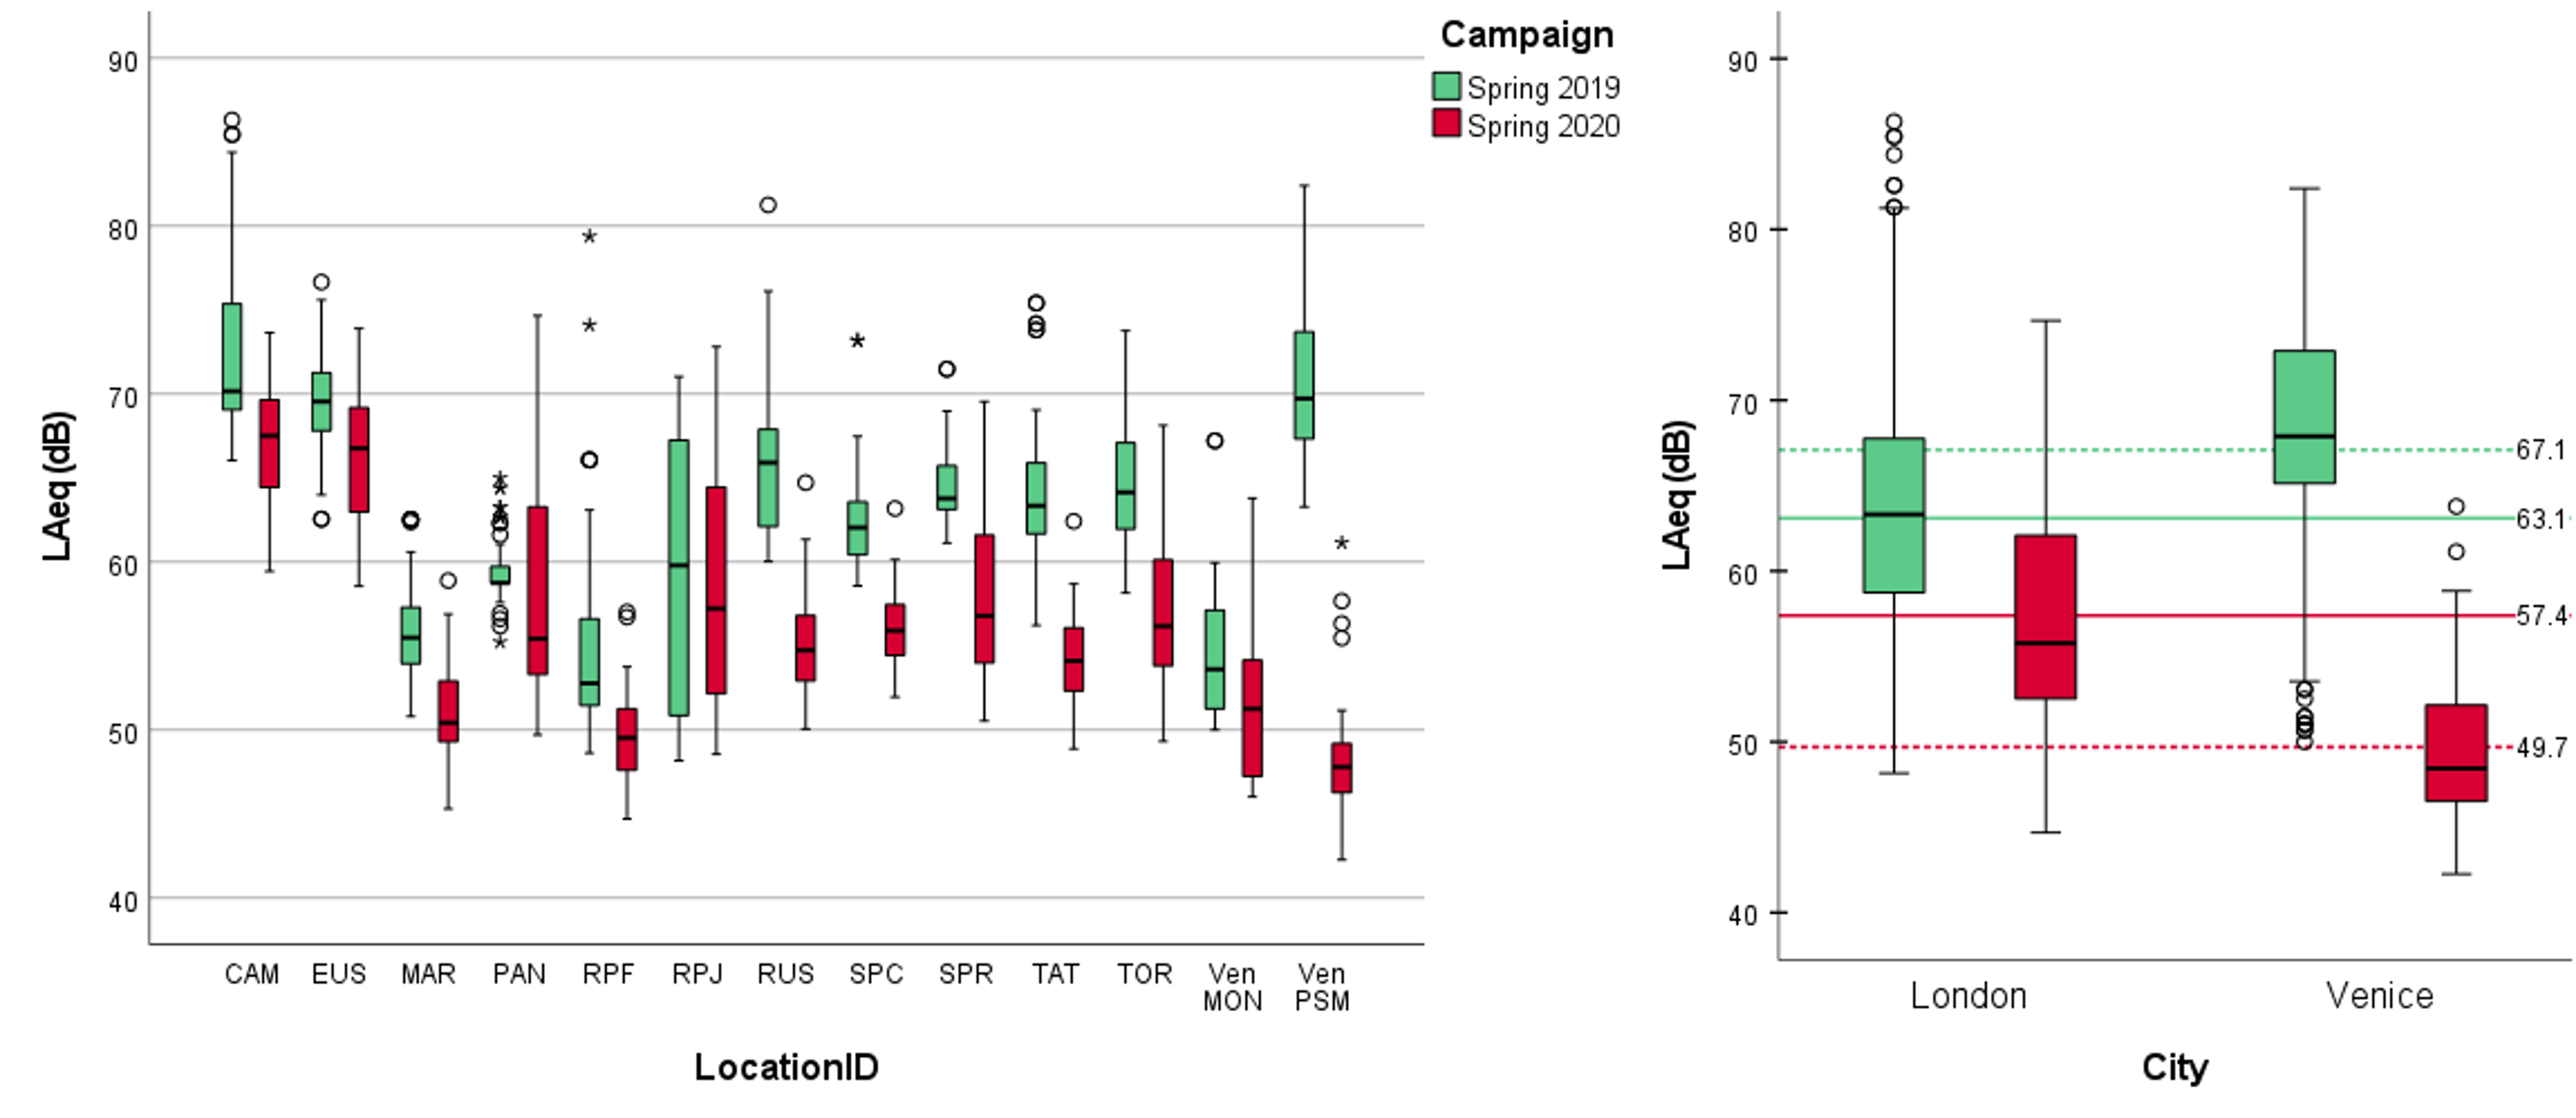
\includegraphics[width=\textwidth]{Figures/LockdownLAeqCombined.png}
  \caption{On the left: Sound levels distributions at the 11 London locations before and during the lockdown measures implementation; on the right: Sound levels distributions in each city (aggregated across locations) and corresponding mean values before and during the lockdown measures implementation (solid line: London; dashed line: Venice). \label{fig:NsMapLockLAeq}}
\end{figure}

%%%%%%%%%%%%%%%%%%%%%%%%%%%%%%%%%%%%%%%%%%%%%%%%%%%%%%%%%%%%%%%%%%%%%%%%

%%%%%%%%%%%%%%%%%%%%%%%%%%%%%%%%%%%%%%%%%%%%%%%%%%%%%%%%%%%%%%%%%%%%%%%%

The t-test results indicate that all locations except Regents Park Japan demonstrate a significant change in the sound environment. Averaged across all locations, sound levels in London and Venice decreased by 5.66 dB and 17.45 dB, respectively, and an overall decrease of 7.08 dB for both cities. In London, the amount of reduction ranges from 10.49 dB (Russell Square) to 1.27 dB (Regents Park Japan). The largest reduction (22.03 dB) is seen in Piazza San Marco which is to be expected given the drastic contextual difference from Carnevale in 2019 to a deserted square in 2020. 

\cref{fig:NsMapLockN5} presents the distributions of \gls{n5} values measured in each of the 13 locations in 2019 and during the lockdown in 2020. The results here closely mirror the \gls{laeq} results. In London the \gls{n5} reduction ranges from 11.03 sones (Russell Square) to 0.35 sones (Pancras Lock). \cref{fig:NsMapLockS} presents the distributions of \gls{s} values measured in each of the 13 locations in 2019 and during the lockdown in 2020. An interesting point here is that, unlike the sound level and loudness results, there was not a universal reduction in the sharpness levels across all locations.

\begin{figure}[h]
  \centering
  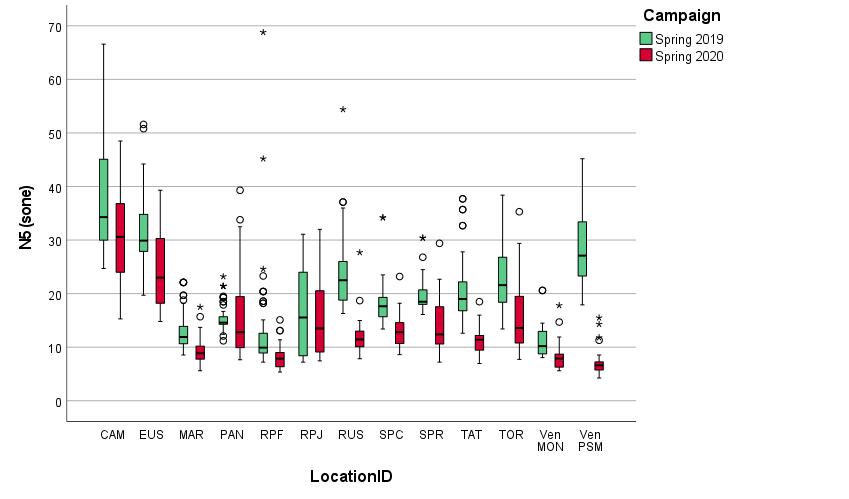
\includegraphics[width=.75\textwidth]{Figures/LockdownLoudness.png}
  \caption{Loudness distributions at the 11 London locations before and during the lockdown measures implementation. \label{fig:NsMapLockN5}}
\end{figure}


\begin{figure}[h]
  \centering
  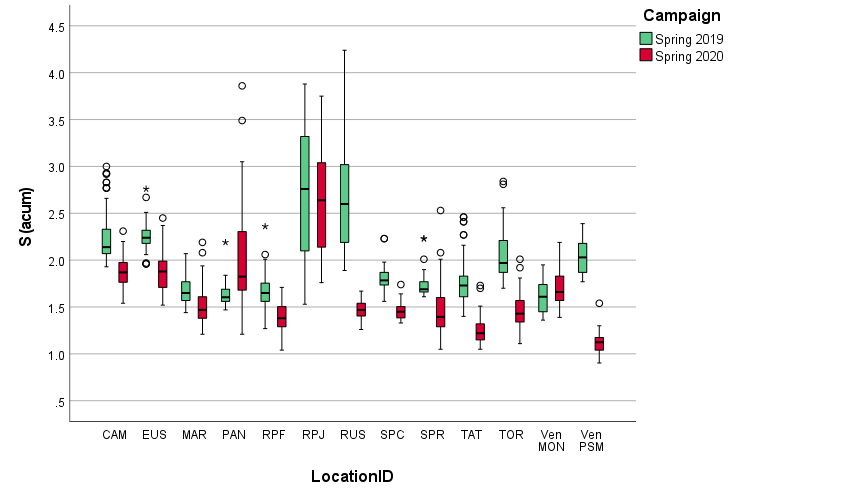
\includegraphics[width=.75\textwidth]{Figures/LockdownSharp.png}
  \caption{Sharpness distributions at the 11 London locations before and during the lockdown measures implementation. \label{fig:NsMapLockS}}
\end{figure}

\paragraph*{Effect of the urban setting on sound levels reduction}

In addition to strictly documenting the changes in the sound environment in London, we also aimed to investigate whether the lockdown measures would result in different sound level reductions depending on the urban scenario (and its composition of sound sources). For this purpose, it was decided to define an `Area type' variable that would serve as a proxy for urban (acoustic) context: a \emph{k}-means cluster analysis was performed on the mean values of \gls{laeq}, \gls{la10}, \gls{la90}, \gls{n5}, \gls{tu}, \gls{fs}, and \gls{s} of the 2019 measurements campaign for the 11 locations, after those have been \emph{z}-score standardized to meet the algorithm criteria. The rationale was that clustering urban areas \emph{a priori} based on their `typical' acoustic climate (hence using only data from 2019) would allow us to see whether there was an association between area type and noise reduction. The algorithm was set to a three-cluster solution, based on visual inspection of the scree plot as reported in \cref{fig:NsMapLockScree} (`elbow method') \citep{KetchenJr.1996application}. The analysis was conducted in \texttt{R} \citep{RCT2018R} and figures were produced using the package \texttt{factoextra} \citep{Kassambara2020factoextra}.

\begin{figure}[!h]
  \centering
  \begin{subfigure}{.75\textwidth}
    \centering
    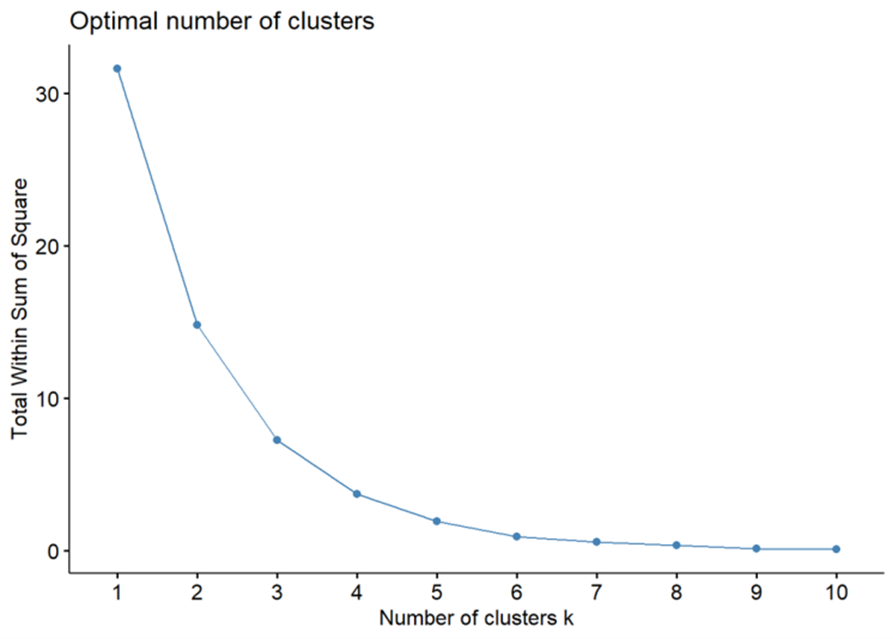
\includegraphics{Figures/NoiseMappingLockdown Fig 6.png}
    \caption{`Scree' plot used to identify the optimal number of clusters to use in the \emph{k}-means clustering algorithm where an `elbow' can be identified for a three-cluster solution. \label{fig:NsMapLockScree}}
  \end{subfigure}
\hfill
  \begin{subfigure}{.75\textwidth}
    \centering
    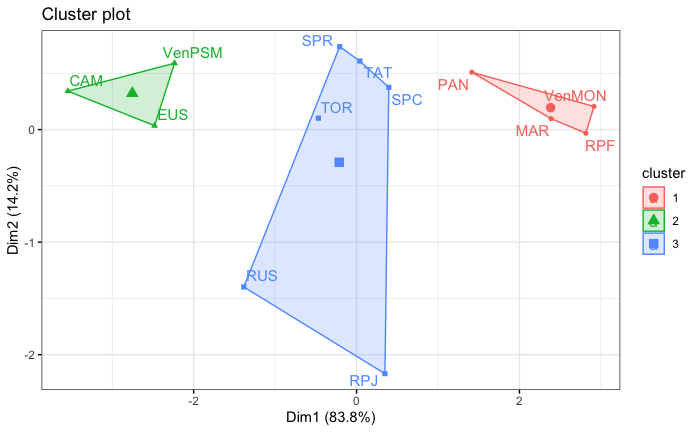
\includegraphics[width=\textwidth]{Figures/LockdownClusterAnalysis1_2022-04-29.png}
    \caption{Bi-dimensional plot for the three-cluster solution. The clusters have been labelled as: Cluster 1 -- Quiet Areas; Cluster 2 -- Active Areas; Cluster 3 -- Traffic/Noise-dominated Areas. \label{fig:NsMapLockBiplot}}
  \end{subfigure}

\caption{Clustering analysis of 2019 prelockdown data.}

\end{figure}

% \begin{figure}[h]
%   \centering
%   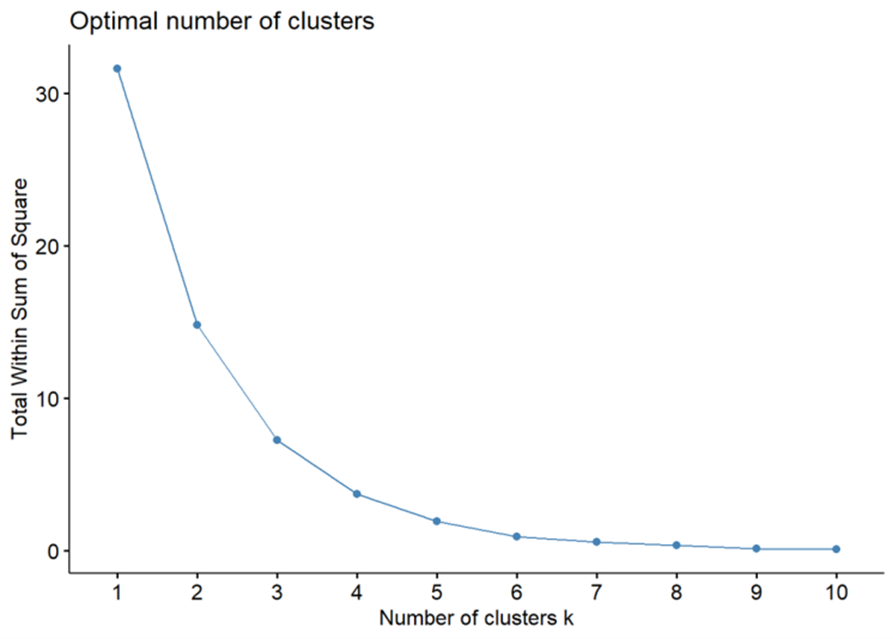
\includegraphics[width=.65\textwidth]{Figures/NoiseMappingLockdown Fig 6.png}
%   \caption{`Scree' plot used to identify the optimal number of clusters to use in the \emph{k}-means clustering algorithm where an `elbow' can be identified for a three-cluster solution. \label{fig:NsMapLockScree}}
% \end{figure}

\cref{fig:NsMapLockBiplot} shows a plot of clustered data based on the two most relevant underlying dimensions for the three-cluster solution. Dimension 1 seems to describe a pattern related to sound level and associated metrics, whilst Dimension 2 is related to Sharpness. This is consistent with previous findings in literature where it was observed that when it comes to categorization and classification of urban acoustic environments based on objective features, most solutions are reduced to intensity- and spectral-related parameters \citep{deCoensel2006quiet,Aletta2017Dimensions}.

\cref{tab:NsMapLockClust} shows the basic descriptive statistics of the psychoacoustic features for the 11 locations according to cluster membership; when combining those patterns with information about dominant sound sources as derived from data from \citet{Mitchell2020Soundscape}, the three clusters could be labelled as: \emph{Traffic/Noise-dominated areas} (locations: Camden Town, Euston Tap, Piazza San Marco), \emph{Active Areas} (locations: Regents Park Japan, Russell Square, St Pauls Cross, St Pauls Row, Tate Modern, Torrington Square) and \emph{Quiet Areas} (locations: Marchmont Garden, Pancras Lock, Regents Park Fields, Monumento Garibaldi). Traffic/Noise-dominated (with the exception of San Marco) areas with an exceptionally high noise level; typically this is because they are on major roads, where traffic noise is the dominant sound source. However Piazza San Marco also clusters here due to its unique use-case. Active areas are locations where the human activity (also combined with traffic) is the main contributor to the acoustic environment. Quiet areas are generally parks or areas with greenery that tend to have a relatively low background noise (lack of traffic sources).

\begin{table}[!h]
  \centering
  \caption{Descriptive statistics of the psychoacoustic metrics for the three identified clusters. \label{tab:NsMapLockClust}}
    \begin{tabular}{llccccc}
      \toprule
      \textbf{Cluster} & \textbf{Parameter} & \multicolumn{5}{c}{\textbf{Mean values }}     \\
      \cline{3-7}      &                    & $L_{Aeq}$ & $L_{A10}$ & $L_{A90}$ & $S$ & $N_5$ \\
      \hline
      1 -- (Quiet areas)  & Mean            & 55.9      & 58.1      & 52.4      & 1.7 & 12.9 \\
      {[}N=3]             & Std. deviation  & 2.6       & 2.5       & 3.1       & 0.0 & 1.8  \\
                          & Variance        & 7.0       & 6.3       & 9.3       & 0.0 & 3.1  \\
      \hline
      2 -- (Active areas) & Mean            & 62.5      & 64.3      & 59.6      & 2.1 & 18.9 \\
      {[}N=6]             & Std. deviation  & 2.3       & 2.5       & 2.3       & 0.4 & 2.5  \\
                          & Variance        & 5.3       & 6.4       & 5.5       & 0.1 & 6.3  \\
      \hline
      3 -- (Traffic-dominated areas) & Mean & 70.4      & 72.9      & 66.1      & 2.4 & 34.1 \\
      {[}N=2]             & Std. deviation  & 1.6       & 1.9       & 0.3       & 0.0 & 4.4  \\
                          & Variance        & 2.4       & 3.6       & 0.1       & 0.0 & 19.8 \\
      \bottomrule
    \end{tabular}

\end{table}

When considering the mean \gls{laeq} reductions between 2019 and 2020 as a function of Area type, it can be observed that they vary across the three clusters, as shown in \cref{fig:NsMapLockRedux}. The biggest reductions are for Active areas (M = 6.6 dB; SD = 3.2 dB), followed by Traffic-dominated areas (M = 4.5 dB; SD = 0.8 dB), and Quiet areas (M = 3.6 dB; SD = 1.9 dB). A possible explanation for this is that road traffic at the selected locations in London is still sustained to some extent (e.g. circulation of public transport, key workers, etc.), while the most significant variation in Active areas is possibly due to the complete lack of (non-motorized) human activity on site. The locations in the cluster labelled as Quiet areas were already not particularly noisy even before the lockdown, thus the small changes observed are probably once again due to the absence of people.

\begin{figure}[h]
  \centering
  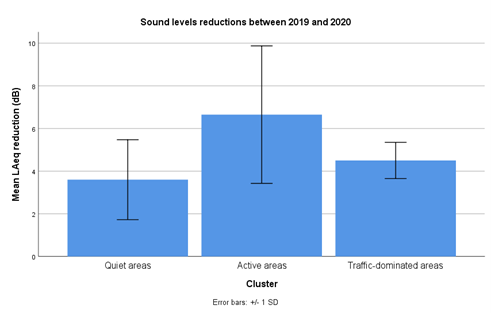
\includegraphics[width=.7\textwidth]{Figures/NoiseMappingLockdown Fig 8.png}
  \caption{Mean A-weighted equivalent sound level reductions between the pre- and during-lockdown conditions as a function of cluster membership (i.e. Area type). \label{fig:NsMapLockRedux}}
\end{figure}

%%%%%%%%%%%%%%%%%%%%%%%%%%%%%%%%%%%%%%%%%%%%%%%%%%%%%

 \subsection{Perceived sound source dominance}

   \subsubsection{2019 sound source composition per location}
  While the previous clustering was focussed on differentiating locations according to their strictly acoustic parameters, the listening test allowed us to also differentiate locations according to their sound source profiles. Based on the results derived from the source-dominance questions in the online listening test, this section presents the differences between the locations. Questionnaire data was collected English, Italian, and Spanish in both cities. Data presented here was aggregated per LocationID.


   \begin{figure}[h]
     \centering
     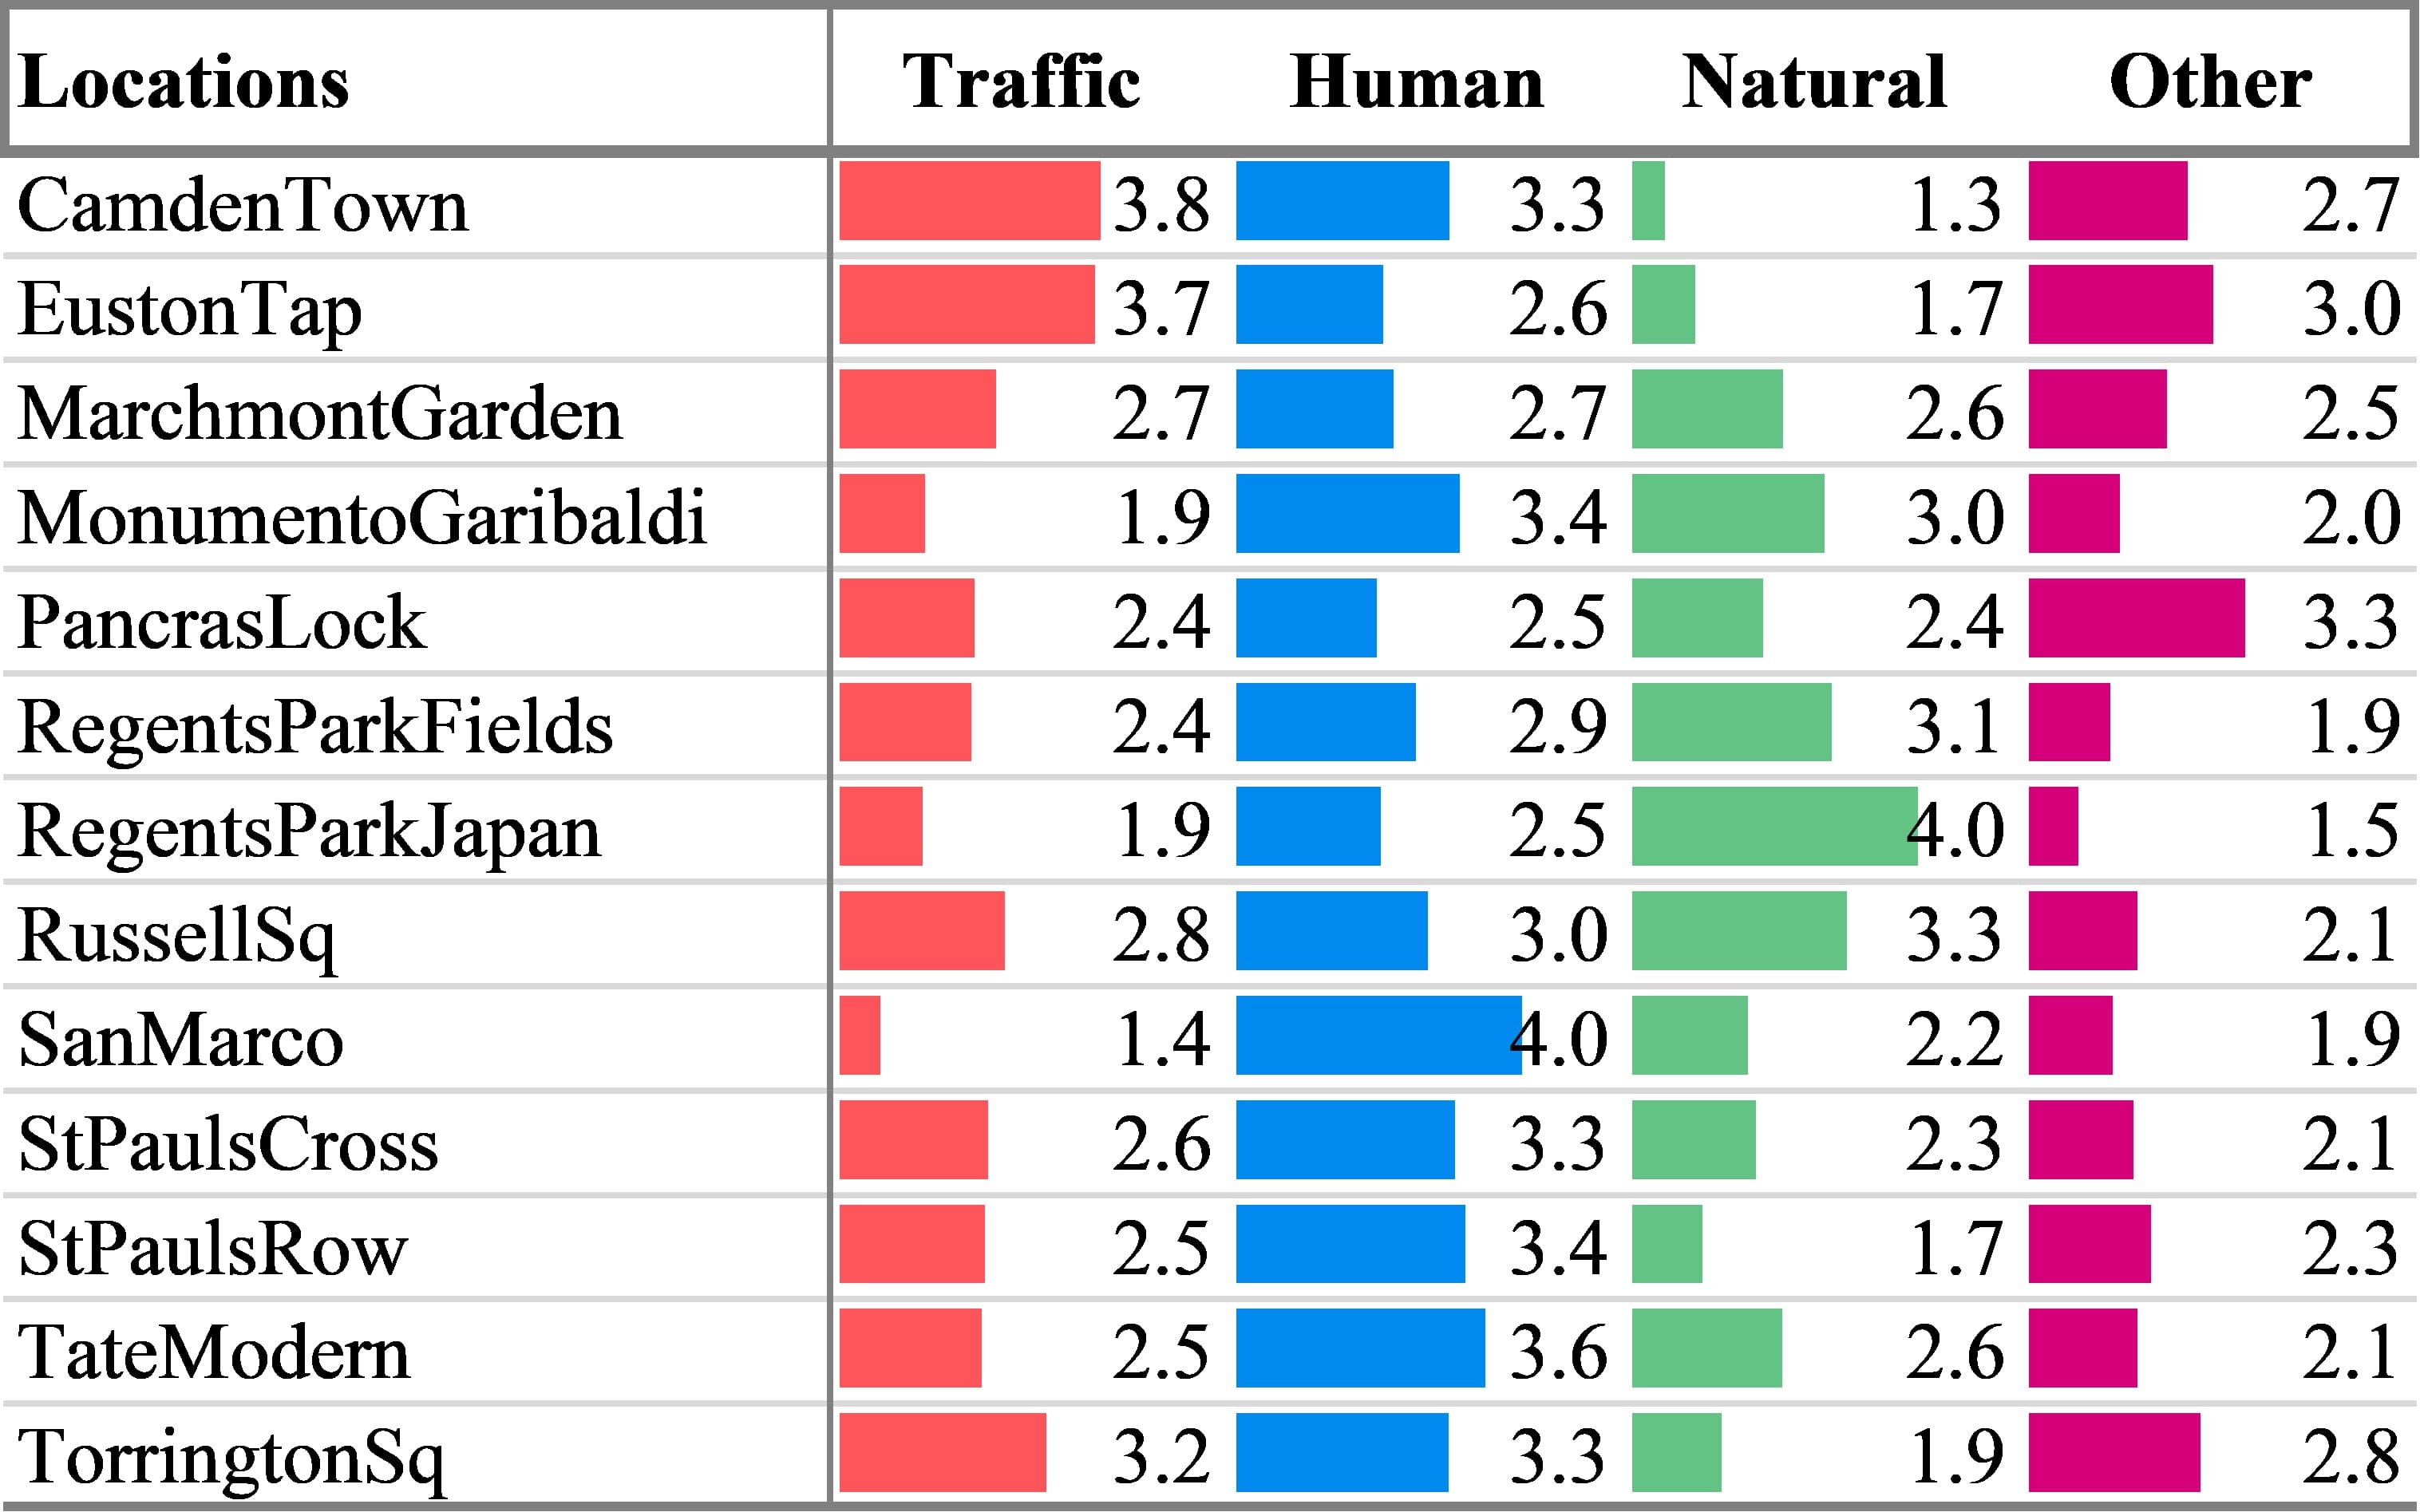
\includegraphics[width=.75\textwidth]{Figures/Lockdown-Fig2.jpg}
     \caption{Mean response per LocationID for the perceived dominance of the sound source types, for the 2019 on-site campaign. The values represent the mean response of all participants in each location to the question `To what extent do you presently hear the following four types of sounds?' Response values range from [1] Not at all to [5] Dominates completely. \label{fig:sound-source-dom}}
   \end{figure}

   According to the highest scored mean value of the dominant sound source type, as shown in \cref{fig:sound-source-dom}, the locations can be grouped into: natural sounds dominated (RegentsParkJapan, RegentsParkFields, RussellSq), human sounds dominated (SanMarco, TateModern, StPaulsRow, StPaulsCross, MonumentoGaribaldi), noise (traffic and other noise) sounds dominated (CamdenTown, EustonTap, TorringtonSq, PancrasLock). Traffic noise and other noise have been combined here and for the rest of the discussion, as these responses are highly correlated within this dataset and it is not helpful to consider them separately for this analysis. This follows the alternative sound source labels given in Fig. C.3 of \citet{ISO12913Part2}, which combines traffic and other noise. Finally, MarchmontGarden is unique in that all of the sound source types are assessed as being nearly equally present with only 0.2 separating the least present (other noise, 2.5) and the most present (traffic noise, 2.7).

   \subsubsection[Overall change in the perceived sound source dominance during lockdown]{Overall change in the perceived sound source dominance during lockdown\footnote{The analysis of the online survey carried out in this subsection was performed by Dr. Tin Oberman. These results are included here verbatim from the original published paper to provide context for the later discussion on the influence of sound source composition on soundscape perception.}}
   \label{sec:soundSourceTin}

    1,803 words describing the sound sources present in the 2019 recordings and 1,395 words related to the 2020 recordings were input by participants in response to the open-ended question Q1 (see \cref{tab:gorilla}). The frequency of occurrence, generated using the WordClouds web application (Wordclouds.com, Zygomatic, Vianen, NL), is shown in \cref{fig:wordclouds}, for the 2019 and the 2020 sets. The highest frequency words from both the 2019 and 2020 groups are: noise, car/traffic, bird/birds, talk/voice, and (foot)steps.


   \begin{figure}[h]
    \begin{subfigure}[b]{0.45\textwidth}
      \centering
      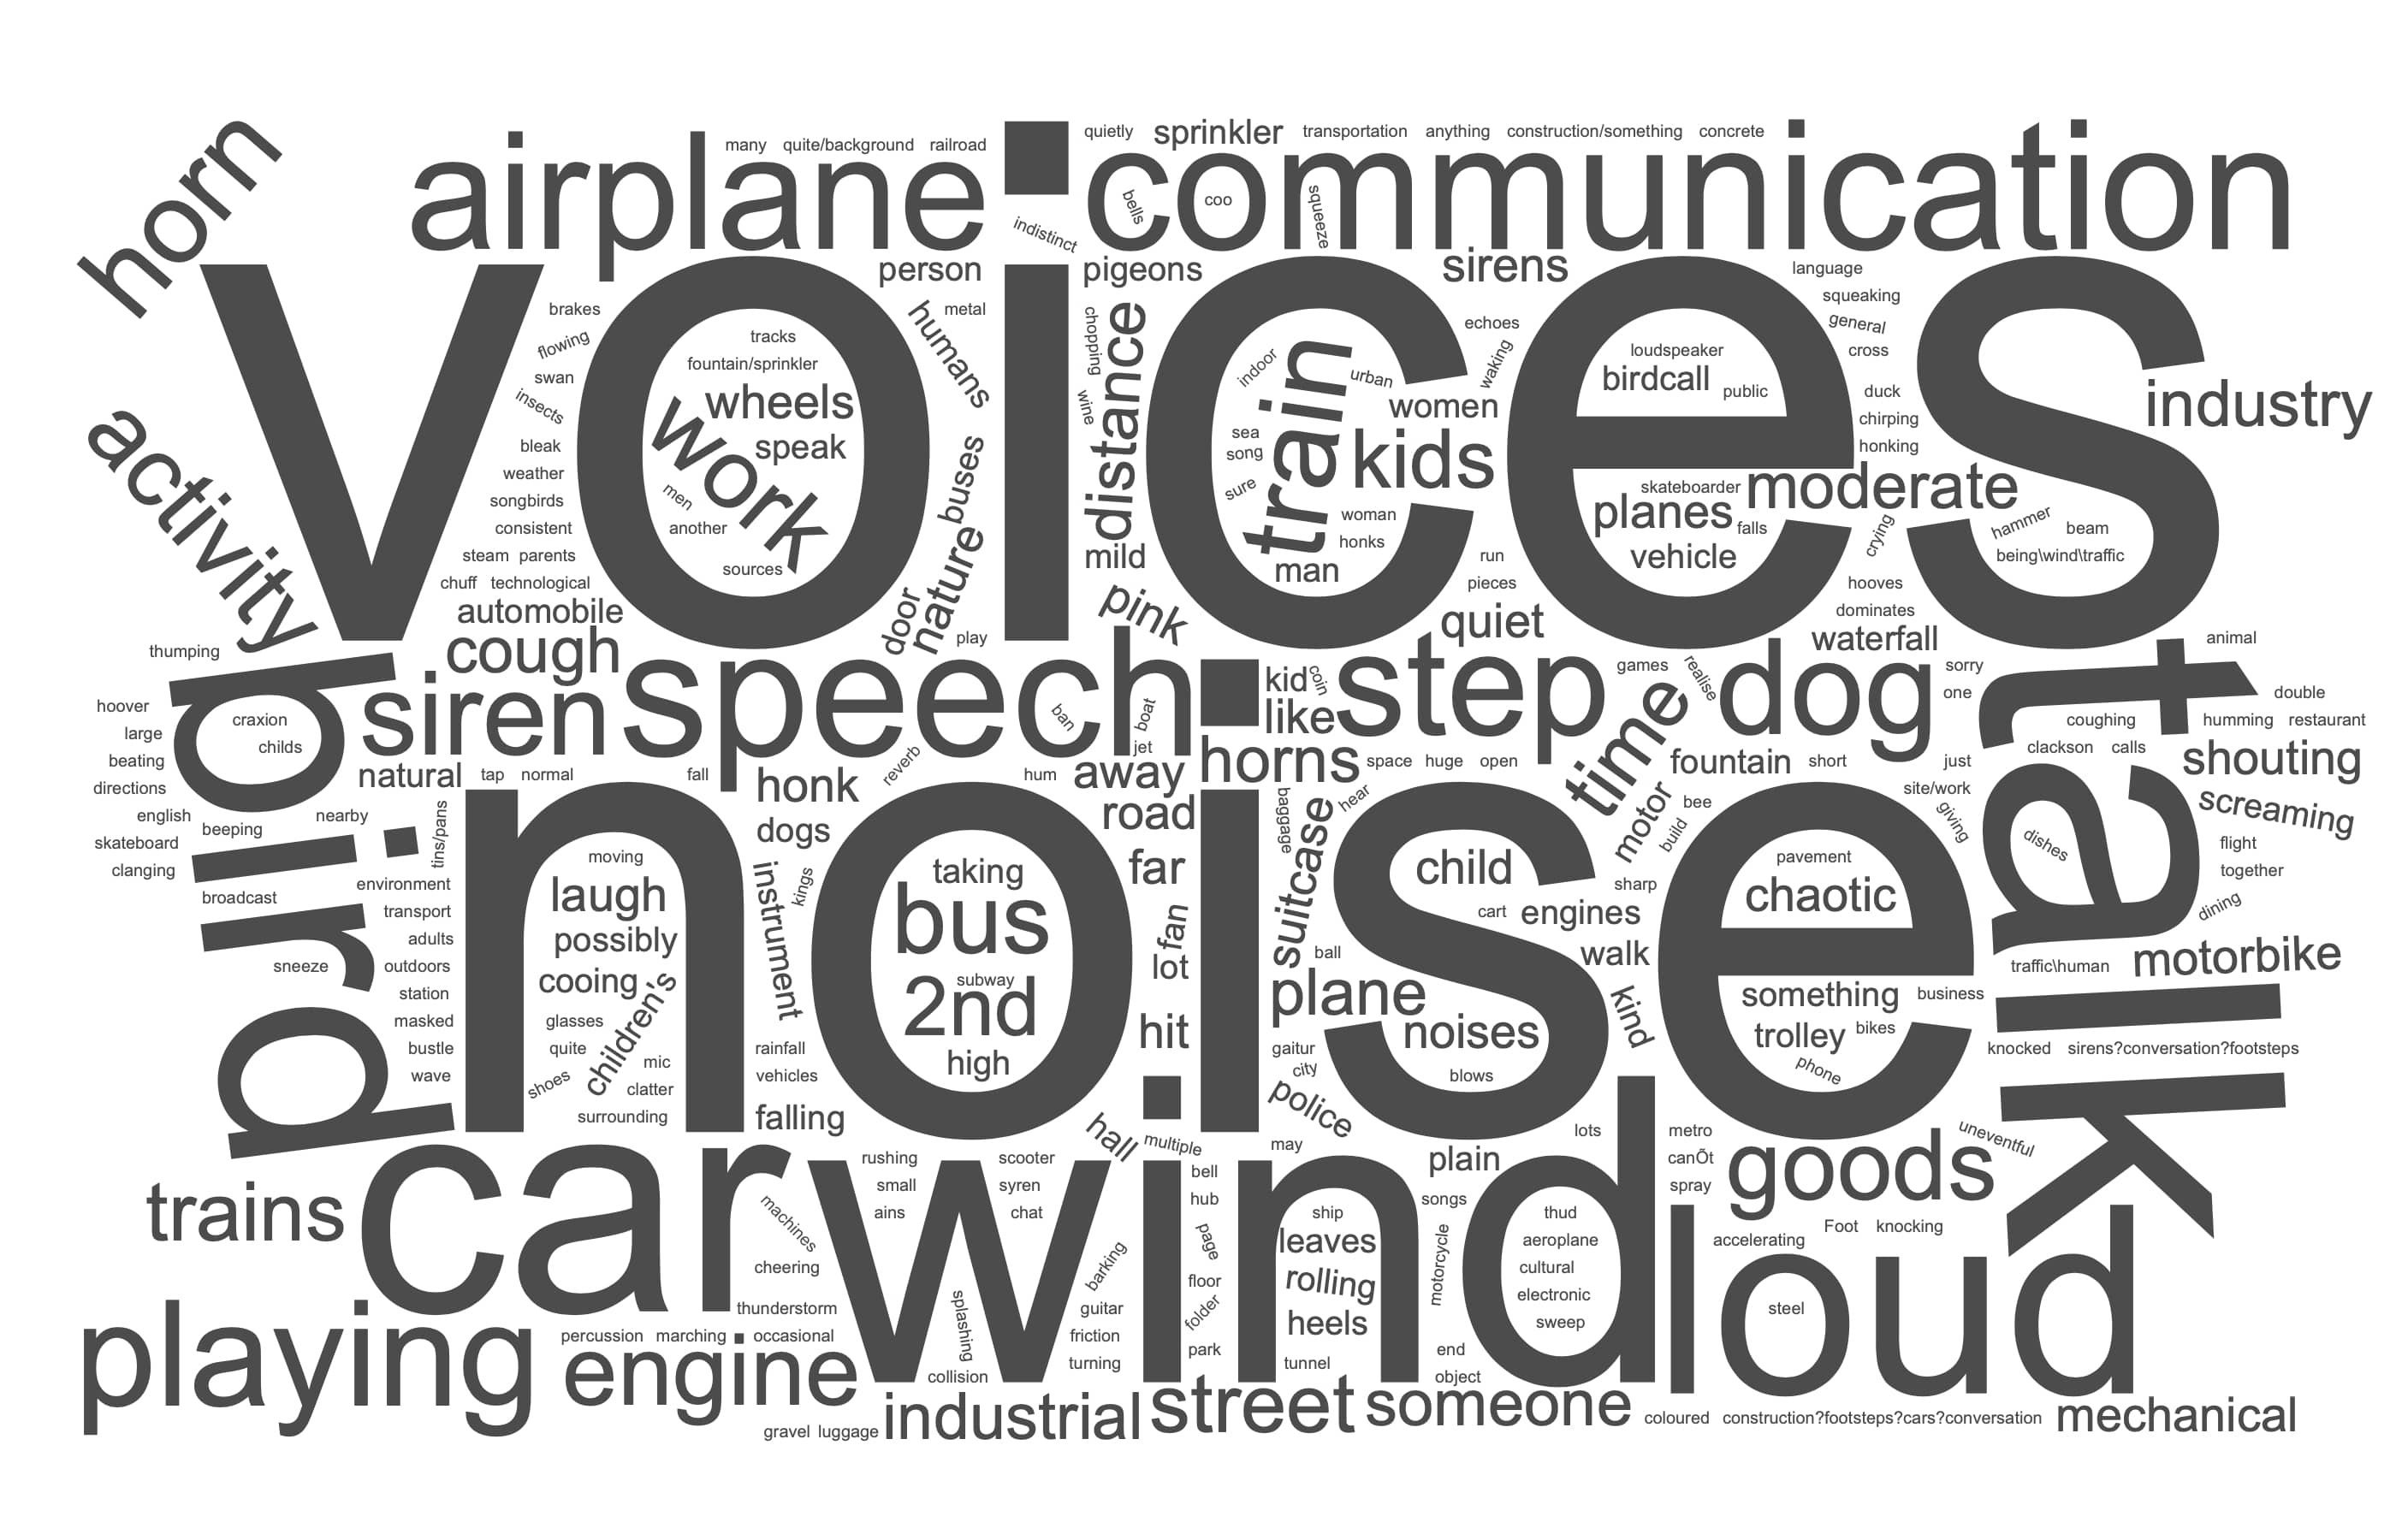
\includegraphics[width=\textwidth]{Figures/Figure3a.jpg}
      \caption{2019 \label{fig:wordcloudA}}
    \end{subfigure}
    \hfill
    \begin{subfigure}[b]{0.45\textwidth}
      \centering
      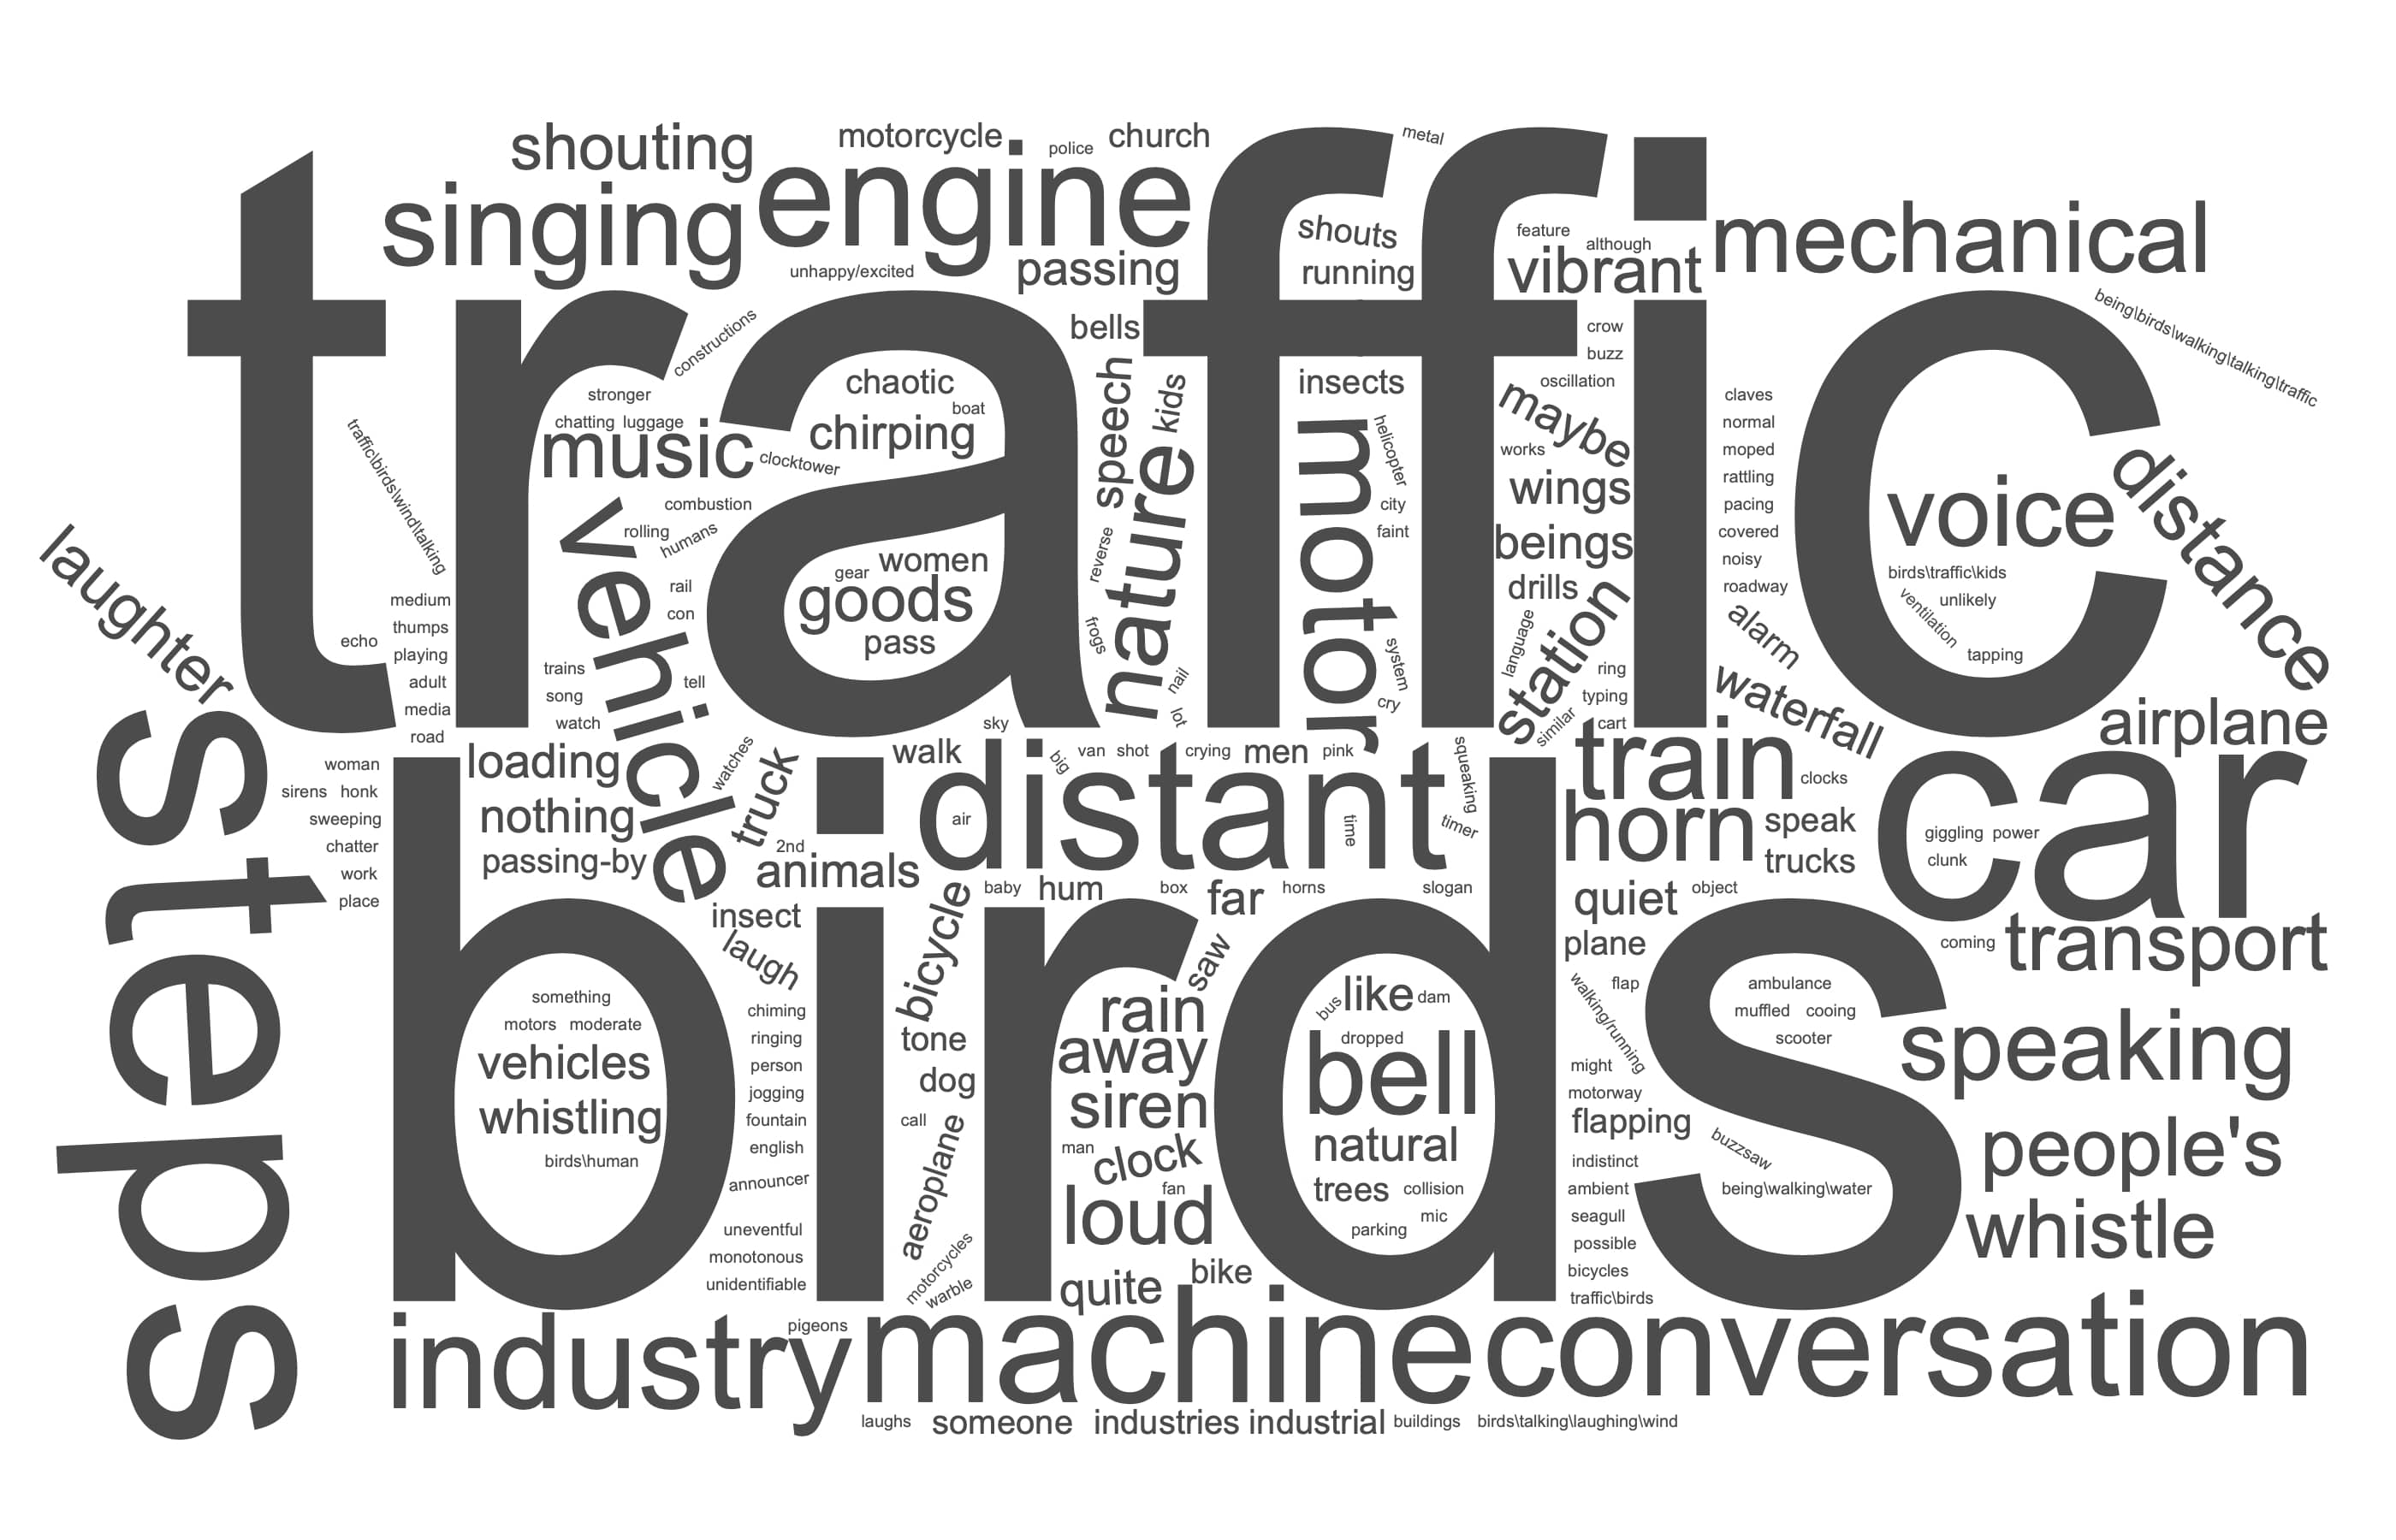
\includegraphics[width=\textwidth]{Figures/Figure3b.jpg}
      \caption{2020 \label{fig:wordcloudB}}     
    \end{subfigure}
    \caption{A graphic illustrating the frequency of occurrence of the sound sources reported by the participants of the online study across all locations, shown for recordings from 2019 (a) and 2020 (b). \label{fig:wordclouds}}
    \end{figure}

   The results from the listening tests deployed online were analysed using SPSS Statistics v. 25 (IBM United Kingdom Limited, Portsmouth, UK; see \cref{tab:source}). Levene's test for equality of variances resulted in highly statistically significant values for all 4 sound sources investigated ($<0.001$). Therefore, a Mann-Whitney U-test was used as a non-parametric equivalent to the t-test to investigate the change in the perceived dominance of the four sound source types \citep{McKnight2010Mann}. The results for human sounds indicated that the perceived dominance was greater for the 2019 sample ($M=3.82$) than for the 2020 sample ($M=2.62, U=41,656, p<0.001$). The results for natural sounds indicated the perceived dominance increased from 2019 ($M=2.00$) to 2020 ($M=2.54, U=63,797, p<0.001$). However, the differences for the noise sources (traffic and other) were not statistically significant. The result of these changes is that although human sounds were the clearly dominant source across the whole dataset in 2019, in 2020, the sound sources are, on average, much more evenly balanced. No single sound source category was identified as frequent across the 2020 dataset.

\begin{table}[h]
\centering
\caption{Mean values and standard deviation for the perceived dominance of sound sources (rated from 1 - 5), assessed via an online survey.}
\label{tab:source}
\begin{tabular}{lccccc} 
\toprule
\textbf{Sound source type} & \textbf{Campaign} & \textbf{N} & \textbf{Mean} & \textbf{Std. Dev.} & \begin{tabular}[c]{@{}c@{}}\textbf{Std. Error }\\\textbf{ Mean}\end{tabular}  \\ 
\midrule
\textbf{Traffic } & 2019 & 422 & 2.51 & 1.369 & .067  \\
                  & 2020 & 383 & 2.56 & 1.525 & .078  \\
\textbf{Other }   & 2019 & 422 & 2.00 & 1.182 & .058  \\
                  & 2020 & 382 & 2.23 & 1.333 & .068  \\
\textbf{Human}    & 2019 & 423 & 3.82 & 1.143 & .056  \\
                  & 2020 & 382 & 2.62 & 1.346 & .069  \\
\textbf{Natural}  & 2019 & 424 & 2.00 & 1.307 & .063  \\
                  & 2020 & 380 & 2.54 & 1.441 & .074  \\
\bottomrule
\end{tabular}
\end{table}

 \subsection{Model selection, performance, and application}

\subsubsection{\gls{isopl} model selected}
   Following the feature selection, the \gls{isopl} model (given in \cref{tab:scaled-model}) has \gls{n5} as the fixed effect with a scaled coefficient of -0.06, and \gls{laeq}, \gls{la10la90}, and \gls{lcla} as coefficients which vary depending on the LocationID. The training and testing \gls{mae} are very similar, indicating that the model is neither over- nor under-fitting to the training data ($MAE_{train}=0.258, MAE_{test}=0.259$), as shown in \cref{fig:lockdownMAE}. The model performs very well at predicting the average soundscape assessment of the locations ($R^2_{train}=0.998, R^2_{test}=0.85$).


   \begin{table}[h!]
  \centering
\caption{Scaled linear regression models of \gls{isopl} and \gls{isoev} for 13 locations in London and Venice. \gls{isopl} model structure: Varying slope, varying intercept multi-level model. \gls{isoev} model structure: Multi-variate linear regression. \label{tab:scaled-model}}

  \def\arraystretch{.5}
   \begin{tabular}{@{}l|cccccc@{}}
    \toprule
    \multicolumn{1}{l|}{} & \multicolumn{3}{c}{\textbf{ISOPleasant}} & \multicolumn{3}{c}{\textbf{ISOEventful}} \\
    \textit{Predictors} & \textit{Estimates} & \textit{CI} & \textit{p} & \textit{Estimates} & \textit{CI} & \textit{p} \\ \midrule
    (Intercept) & 0.24 & 0.15 - 0.33      & \textbf{\textless{}0.001} & 0.14 & 0.12 - 0.16 & \textbf{\textless{}0.001}  \\
    $N_5$      & -0.06 & -0.10 - -0.02 & \textbf{\textless{}0.001} &    &     & \\
    S          &       &               &     & -0.08 & -0.11 - -0.06 & \textbf{\textless{}0.001} \\
    FS         &       &               &     & -0.02 & -0.05 - -0.00 & \textbf{0.033}  \\
    T          &       &               &     & 0.04  & 0.01 - 0.07   & \textbf{0.002}  \\
    $L_{Aeq}$  &       &               &     & 0.14  & 0.11 - 0.17   & \textbf{\textless{}0.001} \\
    $L_{Ceq}-L_{Aeq}$ &  &             &     & -0.03 & -0.05 - 0.00  & 0.052        \\
    \\
    \textbf{Random Effects} &  &       &     &       &               & \\
    $\sigma^2$  & 0.11  &              &     &       &               & \\
    $\tau_{00}$ & \multicolumn{6}{l}{$0.03_{LocationID}$} \\ 
    $\tau_{11}$ & \multicolumn{6}{l}{$0.02_{LocationID.L_{Aeq}}$}  \\
                & \multicolumn{6}{l}{$0.00_{LocationID.L_{A10}-L_{A90}}$} \\
                & \multicolumn{6}{l}{$0.00_{LocationID.L_{Ceq}-L_{Aeq}}$} \\
    ICC         & 0.90 &               &     &       &               &    \\ \midrule
    N           & \multicolumn{6}{l}{$13_{LocationID}$} \\
    Observations & 914 &               &     & 914   &               &  \\
    MAE Test, Train & 0.258 & 0.259    &     & 0.233 & 0.231 \\
    \bottomrule
  \end{tabular}
\end{table}

\begin{figure}[h]
  \centering
  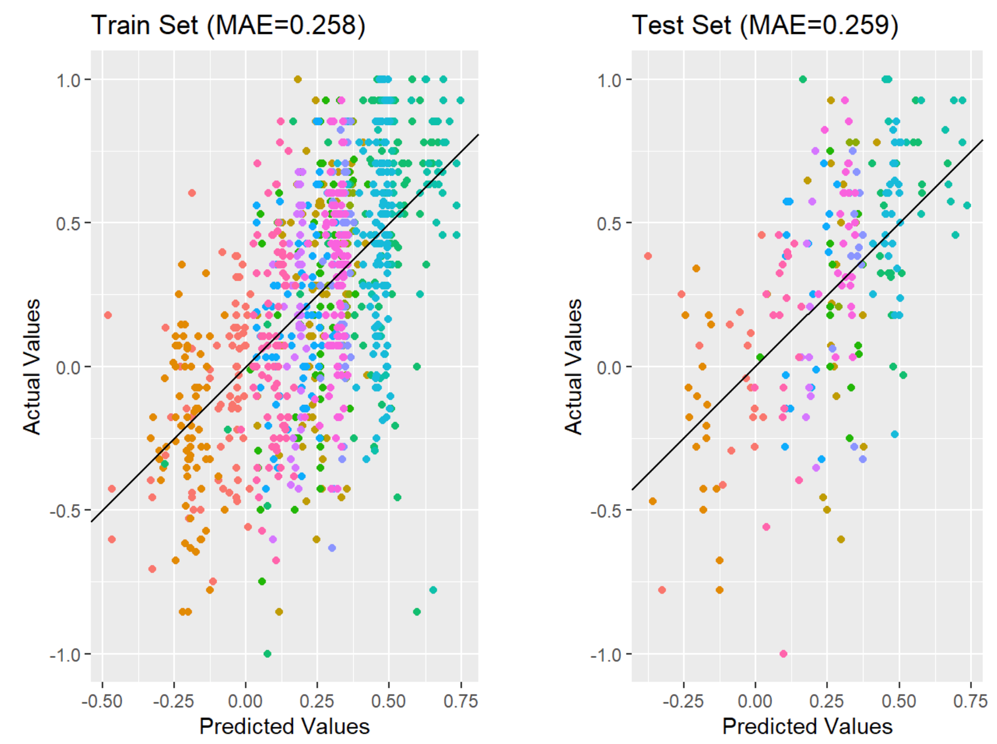
\includegraphics[width=.8\textwidth]{Figures/LockdownMAEPleasnt.png}
  \caption{Scatterplots of the training and testing set prediction results for the \gls{isopl} model. \label{fig:lockdownMAE}}
\end{figure}

   The high intraclass correlation ($ICC=0.90$) demonstrates that the location-level effects are highly important in predicting the pleasantness dimension. Within this varying-intercept varying-slope model structure, these effects include both the specific context of the location (i.e. the LocationID factor), but also the \gls{laeq}, \gls{la10la90}, and \gls{lcla} features whose effects vary across locations. These slopes are given in \cref{fig:pl-slopes}. This point highlights the need to consider how the context of a location will influence the relationship between the acoustic features and the perceived pleasantness.

   \begin{figure}[h]
     \centering
     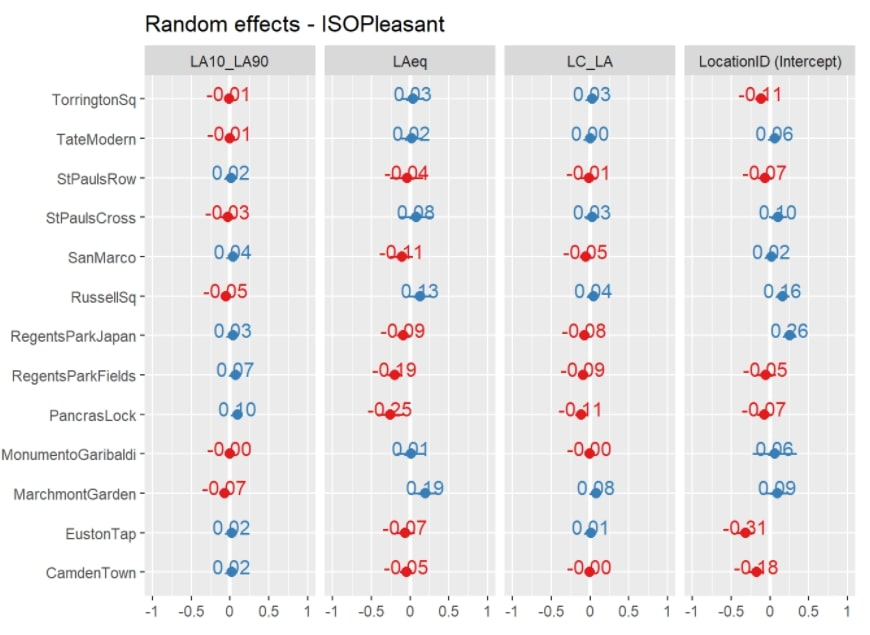
\includegraphics[width=\textwidth]{Figures/Lockdown Figure4.jpg}
     \caption{Location-level scaled coefficients for the \gls{isopl} model. \label{fig:pl-slopes}}
   \end{figure}

   \subsubsection{\gls{isoev} model selected}

   Through the group-level feature selection, all of the group-level coefficients were removed, including the LocationID factor itself. Therefore the final \gls{isoev} model is a `flat' multi-variate linear regression model, rather than a multi-level model. The \gls{isoev} is a linear combination of \gls{s}, \gls{fs}, \gls{tu}, \gls{laeq}, and \gls{lcla}. The training and testing \gls{mae} are very similar, indicating that the model is not over-fit to the training data ($MAE_{train}=0.233; MAE_{test}=0.231$). The model performs slightly worse than the \gls{isopl} at predicting the mean location responses, but still performs well ($R^2_{train}=0.873; R^2_{test}=0.715$).

   \subsubsection{Application to lockdown data}
   \label{sec:applicationLockdown}
   Once the two models were built and assessed, they were then applied to the lockdown recording data to predict the new soundscape ISO coordinates. \cref{fig:prelockdownCircCoordsA} shows the pre-lockdown ISO coordinates for each location and \cref{fig:lockdownCircCoordsB} shows how the soundscapes are predicted to have been assessed during the lockdown period. As in the model assessment process, the predicted responses are calculated for each recording individually, then the mean for each location is calculated and plotted on the circumplex.

   In 2019 the majority of locations in the dataset fall within the `vibrant' quadrant of the circumplex, particularly those which are primarily dominated by human activity (e.g. SanMarco, TateModern). Camden Town and Euston Tap, which are both in general visually and acoustically dominated by traffic, are the only two to be rated as `chaotic', while no locations are, overall, considered to be `monotonous'. During the 2020 lockdown, there is a general positive move along the `pleasant' dimension and a general negative move along the `eventful' dimension, but several patterns of movement can be noted. These are investigated further in the \cref{sec:lockdownDiscussion} below.

\begin{figure}[!hp]
  \centering
  \begin{subfigure}[]{.7\textwidth}
    \centering
    \caption{Prelockdown Location Means \label{fig:prelockdownCircCoordsA}}
    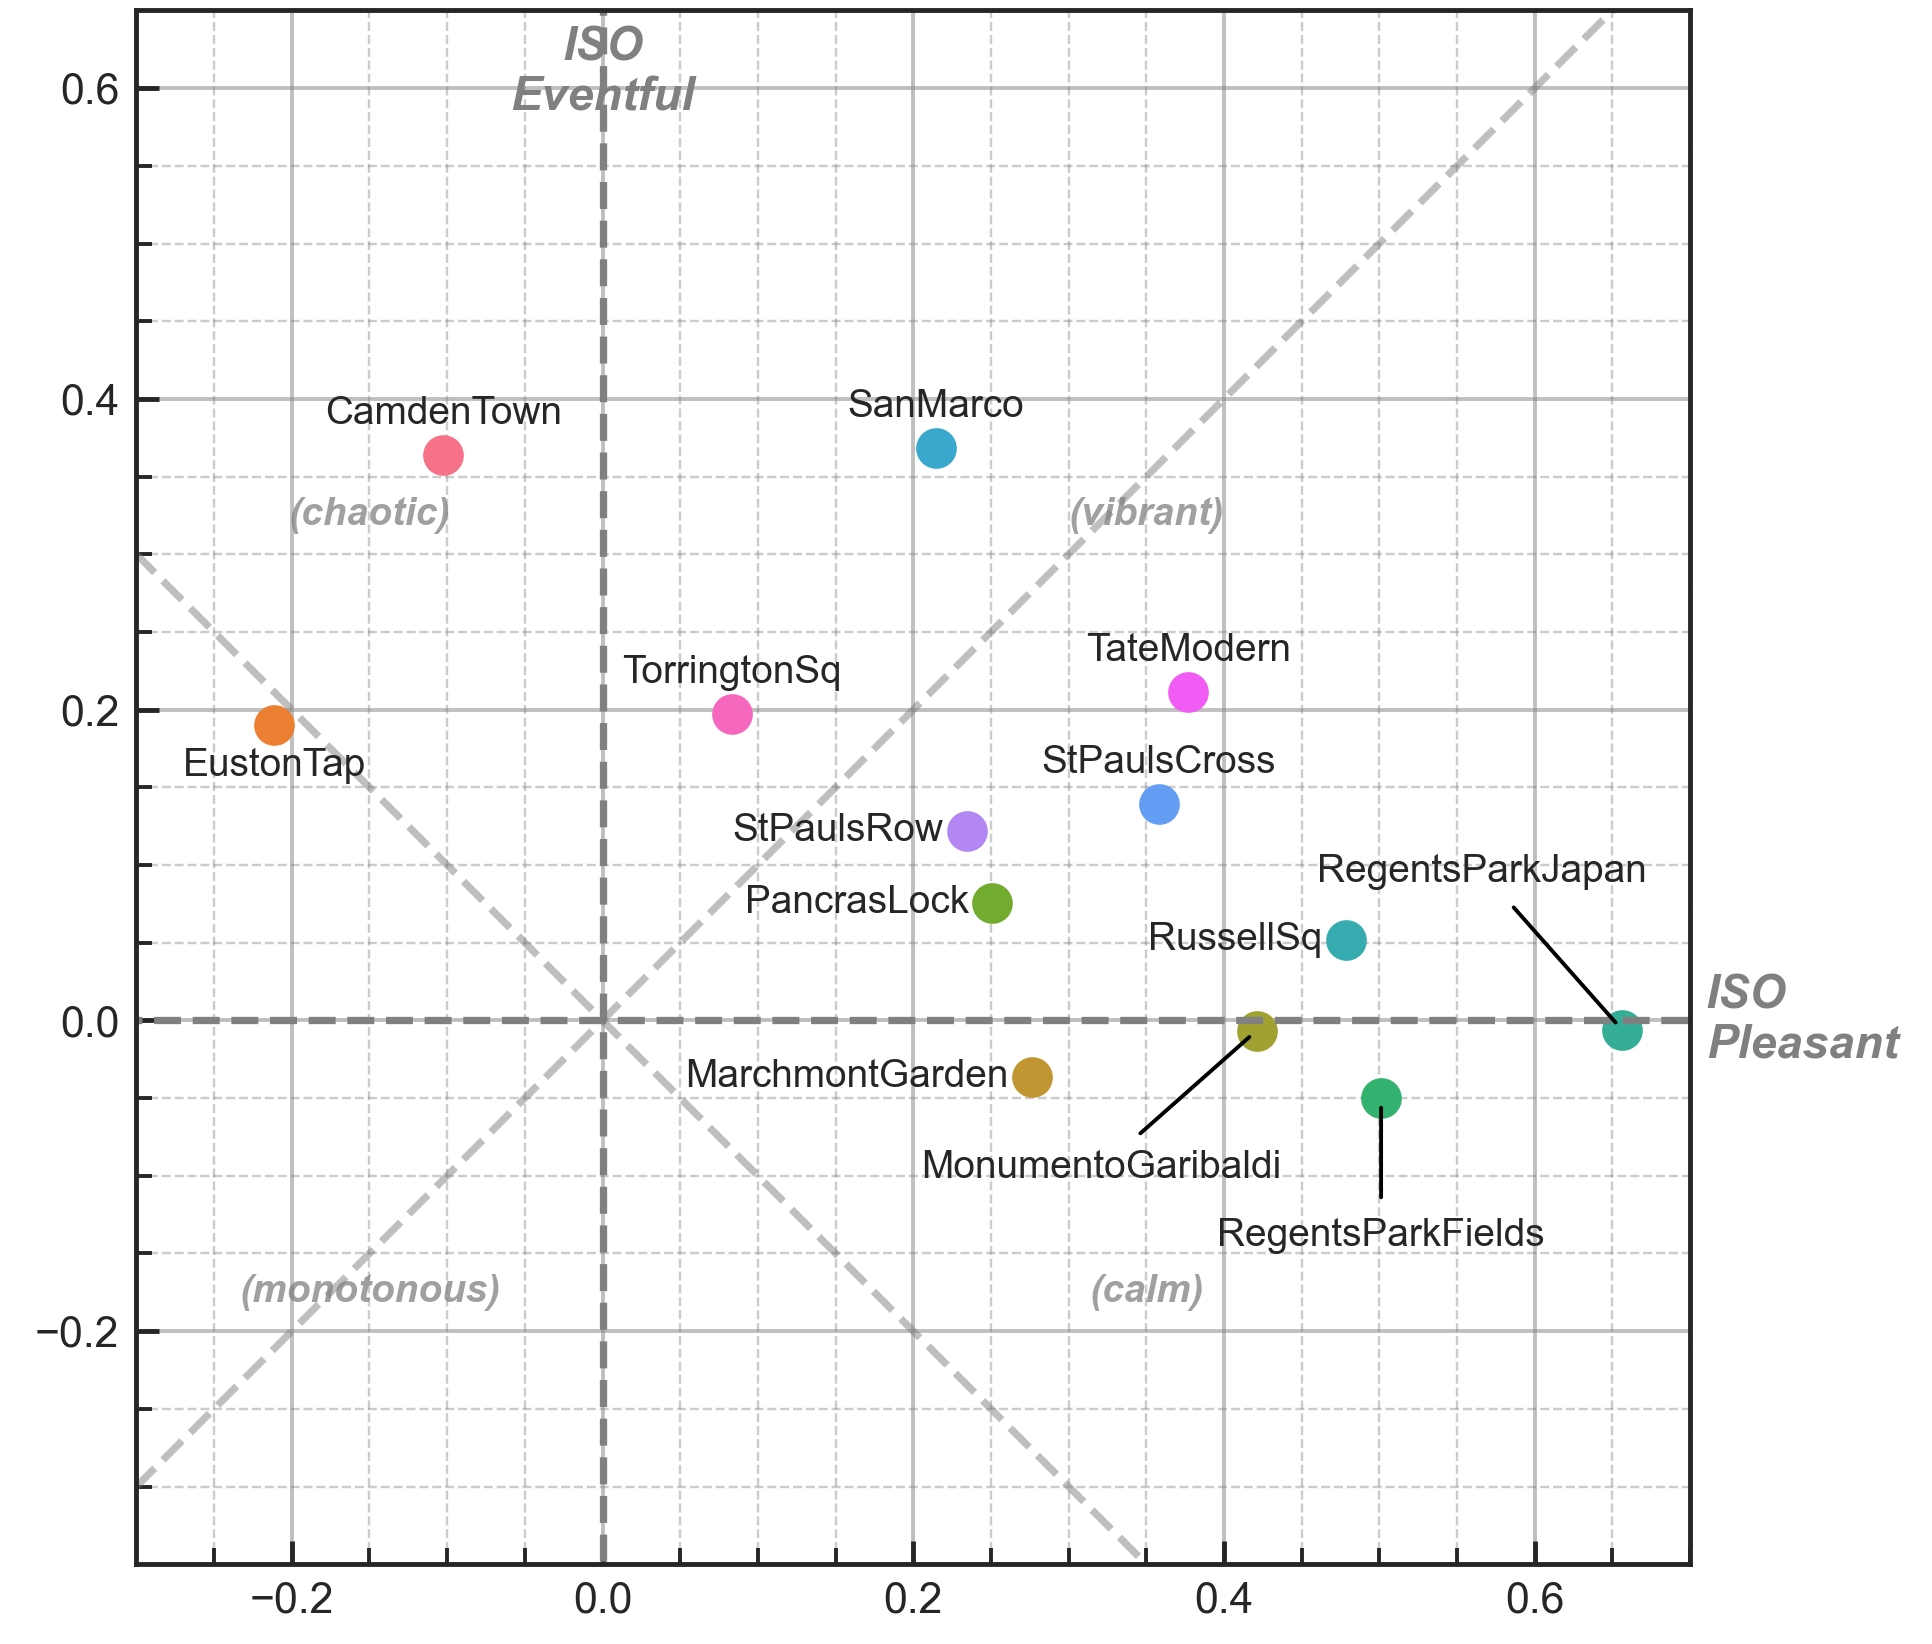
\includegraphics[width=\textwidth]{Figures/LockdownCircCoordsA.jpg}
  \end{subfigure}
  \hfill

  \begin{subfigure}{.7\textwidth}
    \centering
    \caption{Lockdown Location Means (Predicted) \label{fig:lockdownCircCoordsB}}
    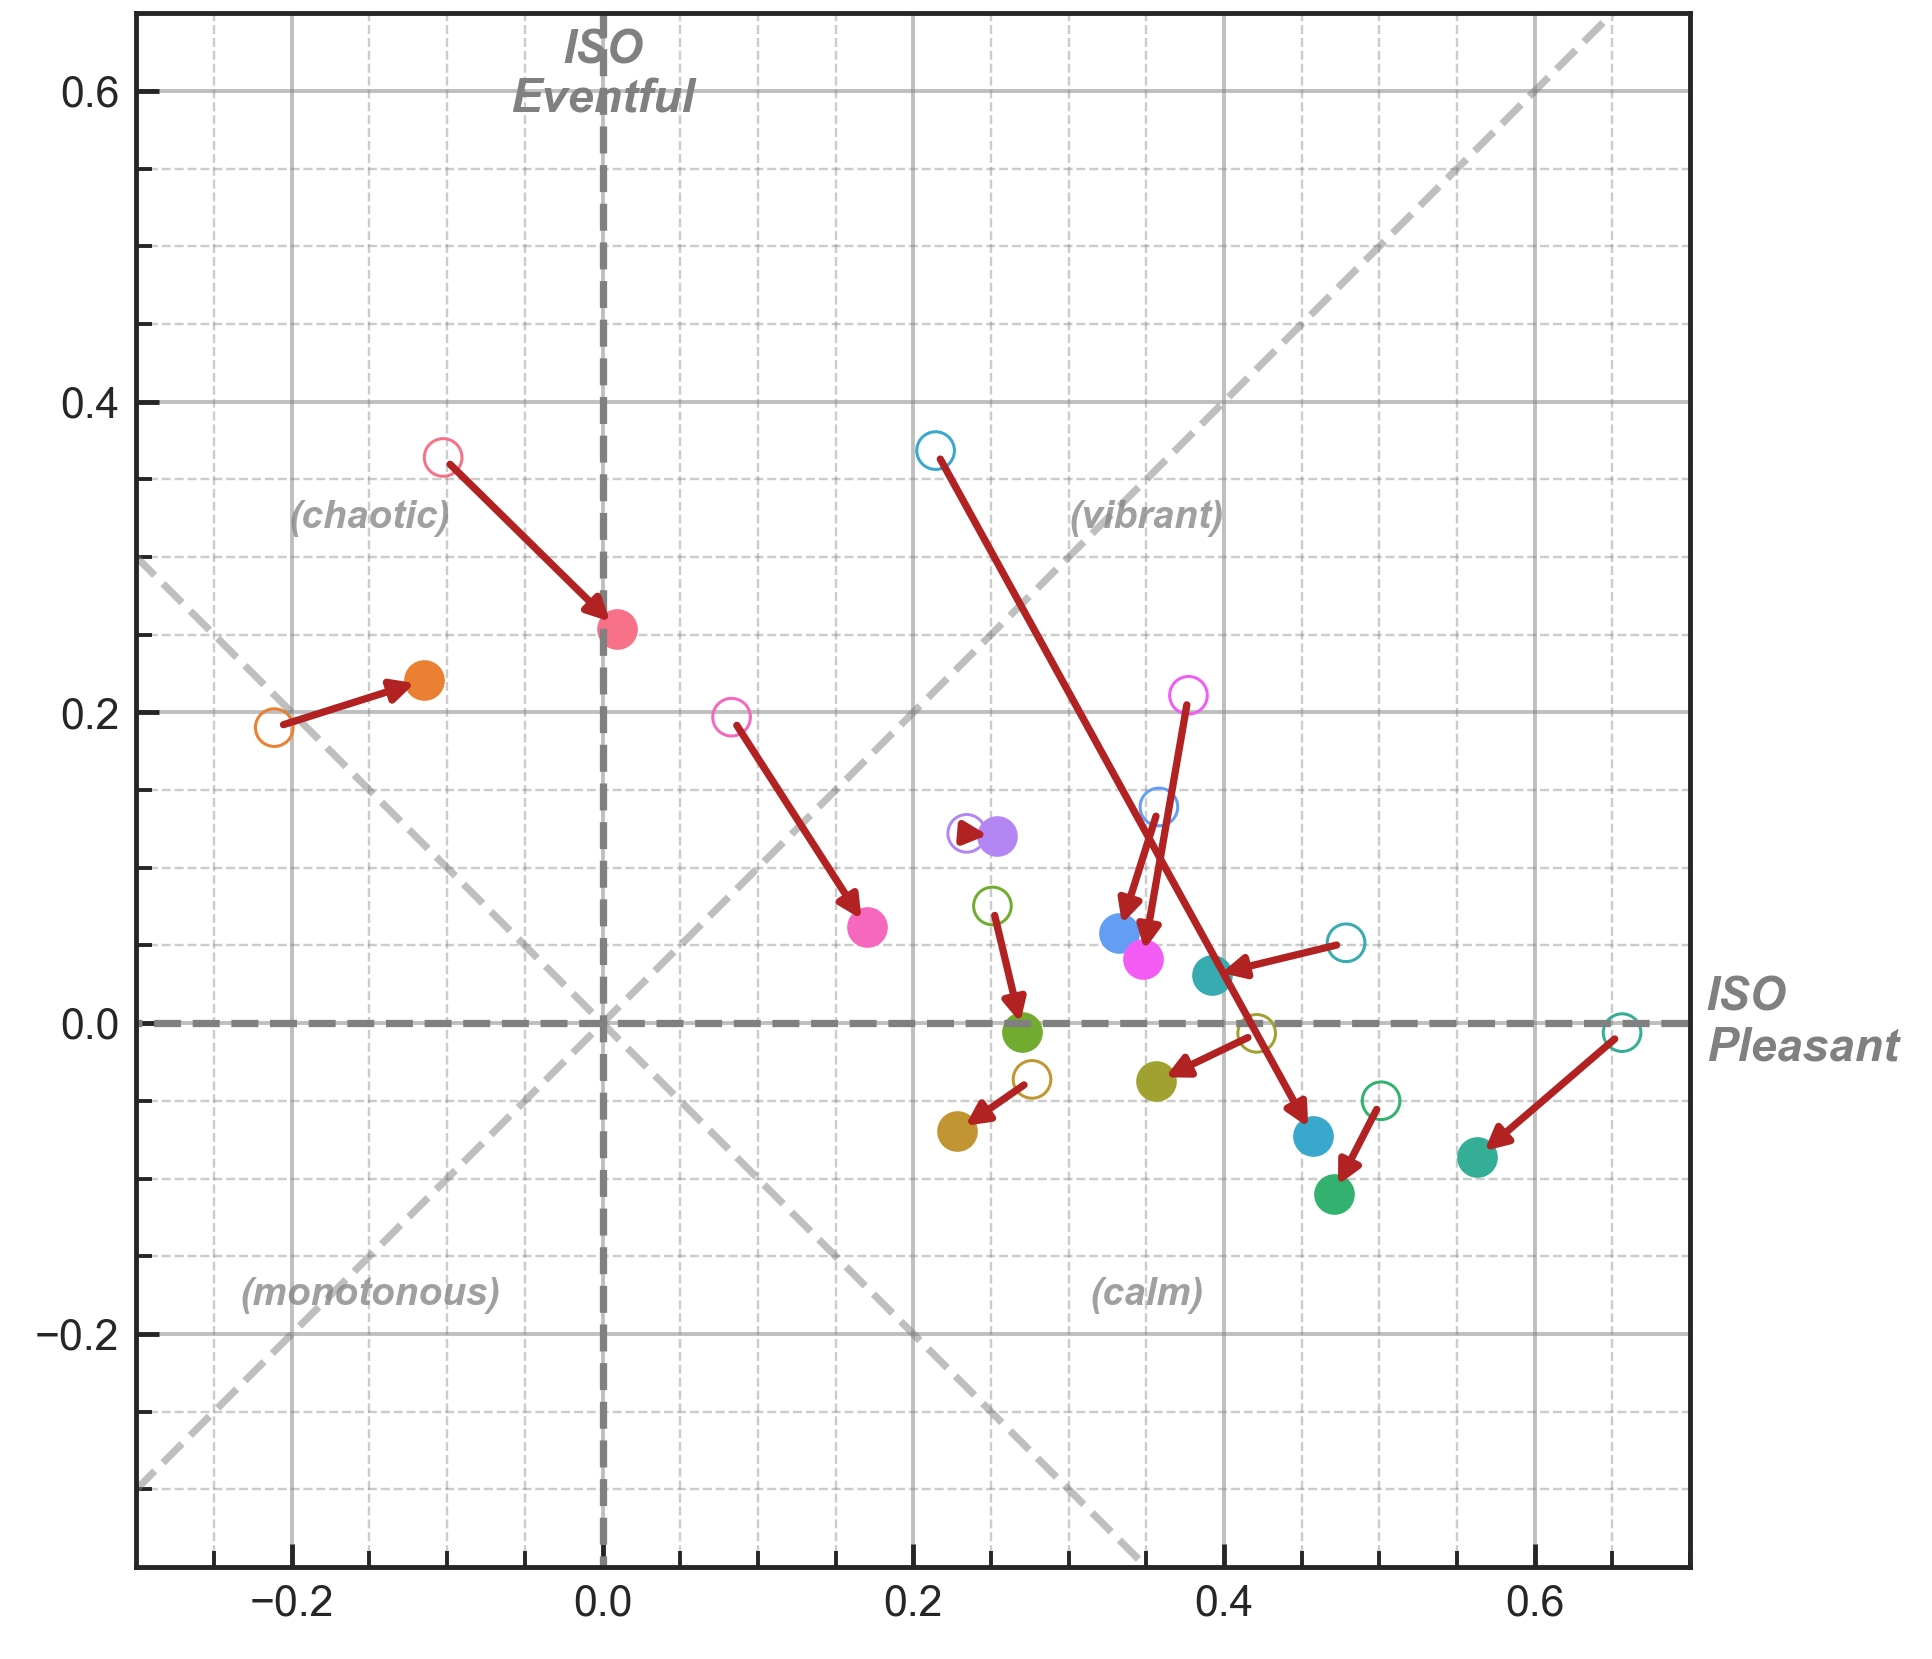
\includegraphics[width=\textwidth]{Figures/LockdownCircCoordsB.jpg}
  \end{subfigure}
  \hfill
  
  \caption{Soundscape circumplex coordinates for (a) the mean \gls{isopl} and \gls{isoev} responses for each location; and (b) the mean predicted responses based on recordings made during the lockdown and the change in the location's placement in the circumplex. In (b) the marker outline is shown for the 2019 location, red arrows indicate the change in the location's coordinates. \label{fig:circumplex-locations}}
  
\end{figure}

%%%%%%%%%%%%%%%%%%%%%%%%%%%%%%%%%%%%%%%%%%%%%%%%%%%%%%%%%%%

\section{Discussion}
\label{sec:lockdownDiscussion}
 \subsection{Interpretation of the results}

   To interpret the results addressing RQ1\footnote{RQ1: How would people have perceived these outdoor urban spaces as a result of this change in acoustic environment?} and RQ2\footnote{RQ2: Would these sound level reductions result in improvements to the soundscape of the spaces?}, it is necessary to separately look into the overall change in sound source composition, and the change in the affective quality of soundscapes per location.

   \subsubsection{Change in the sound source composition}

   The open-ended question about sound sources in the online survey did not reveal a change in sound source types but rather confirmed that all types were still present in both conditions. The sound source composition question taken from the Method A of the ISO/TS 12913-2:2018 \citep{ISO12913Part2} revealed a statistically significant reduction in human sound sources and a significant increase in the perceived dominance of natural sound sources.

   The most frequent sound sources detected from the open-ended question correspond to the main four sound source types investigated, which indicated that all types remained present in the lockdown condition (at all the locations). While traffic intensity might have gone down, where the results of the Mann-Whitney \emph{U}-test were inconclusive, but supported by the psychoacoustic measurements according to \citet{Aletta2020Assessing}, traffic-related sound sources were still clearly present.

   The sound source composition of an outdoor acoustic environment is extremely complex. Removing one component, such as human sounds, has implications on the whole soundscape \citep{Gordo2021Rapid}. Testing the effects of this \emph{in-situ} is not straightforward; interpreting this study in line with `what is the impact of human sounds' must be taken within the broader context of the range of conditions which changed within the acoustic environment. However, looking at the overarching picture, the lockdown condition was a useful and unique case study to understand the impact which human activities -- and the human sound source type in particular -- can have on soundscape perception of urban open spaces.

   \subsubsection{Predicted relative changes in soundscapes due to \gls{covid19} restrictions}

%%%%%%%%%%%%%%%%%%%%%%%%%%%%%%%%%%%%%%%%%%%%%%%%%%%%%%%%%%%

   \begin{figure}[!h]
    \centering
    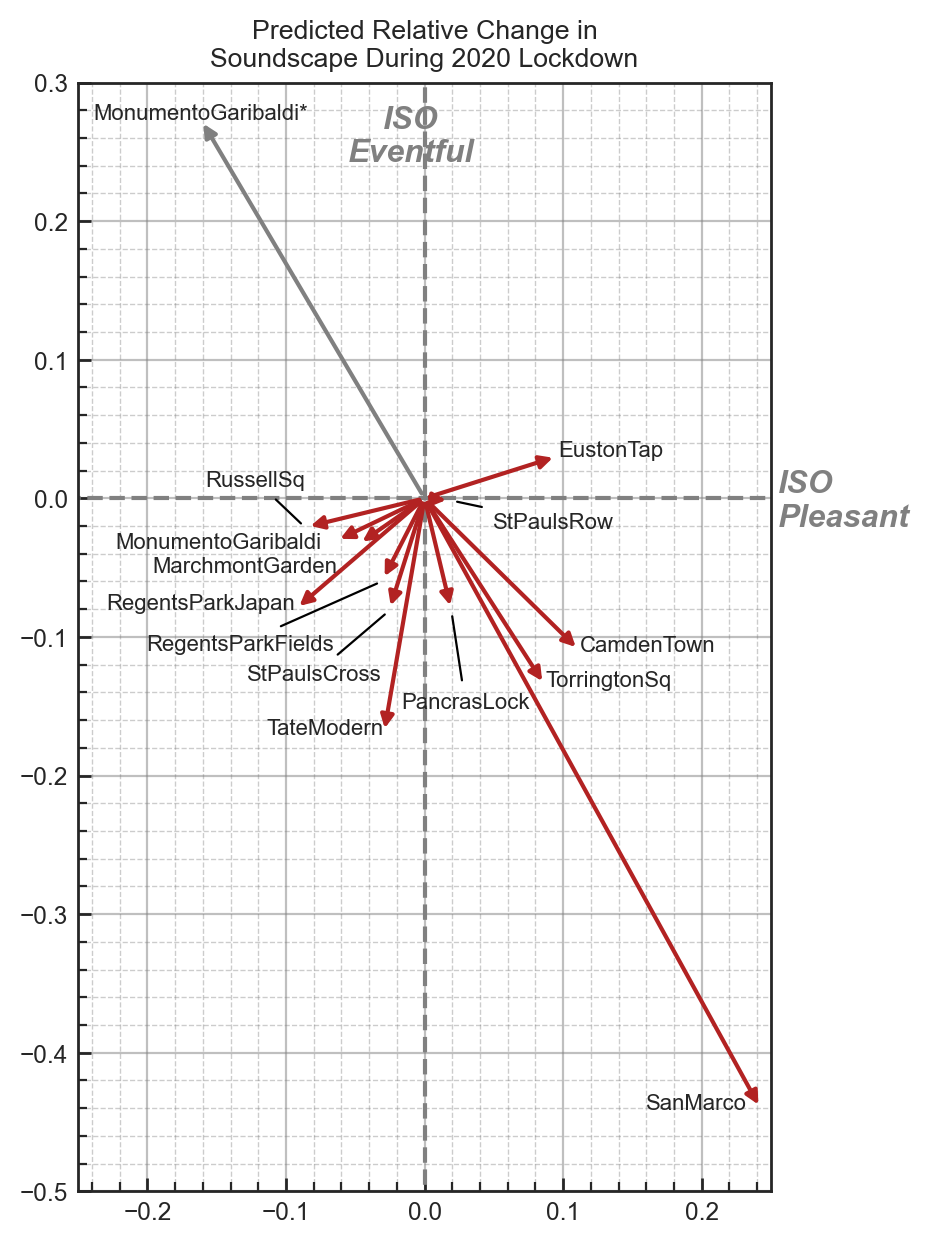
\includegraphics[width=.75\textwidth]{Figures/Lockdown Figure6.jpg}
    \caption{The relative change in soundscape perception in the circumplex due to the \gls{covid19} lockdowns as predicted by the models, represented as vectors centred on the origin. *The lawn-works dominated session is shown separately as MonumentoGaribaldi* with a grey arrow to indicate that this is distinct from the effects of the lockdown changes. \label{fig:circumplex-vectors}}

   \end{figure}

%%%%%%%%%%%%%%%%%%%%%%%%%%%%%%%%%%%%%%%%%%%%%%%%%%%%%%%%%%%

   To interpret how the change of the acoustic environment at the locations examined would have been perceived, and to answer RQ2, relative change vectors within the circumplex space are shown in \cref{fig:circumplex-vectors}. This clearly shows a few different patterns of soundscape change due to the effects of the 2020 lockdown. These can be further looked into depending on the magnitude and direction change; shifts between the quadrants, show in \cref{fig:circumplex-locations}; and the sound source composition. The discussion below is organised according to groups to locations which show similar behaviours in the predicted magnitude and direction of the change, or discusses a single location that is particularly notable.

   \paragraph{Piazza San Marco} The largest change is seen in Piazza San Marco, with a predicted increase in pleasantness of 0.24 and a decrease in eventfulness of 0.44, enough to move the soundscape out of the `vibrant' quadrant and into `calm'. This extreme change (relative to the rest of the locations) is exactly what would be expected given the unique context of the measurements taken in 2019 -- the measurement campaign corresponded with Carnevale, a yearly festival which centres around the square. By contrast, due to the particularly strict measures imposed in Italy, during the lockdown measurement period the square was almost entirely devoid of people. What is promising is that, without any of this contextual information about the presence or absence of people, my model is able to capture and reflect what may be considered a reasonable and expected direction and scale of change within the soundscape circumplex.

   \paragraph{Locations showing an increase in pleasantness} The next locations of interest are those which, in the 2019 survey data, were rated as being dominated by traffic noise: Euston Tap, Camden Town, Torrington Square, and Pancras Lock. These are the only locations (besides San Marco) which show a predicted increase in pleasantness. Of these traffic-dominated spaces, the two which were most heavily dominated by traffic noise (Camden Town and Euston Tap) showed the most increase in pleasantness, with Torrington Square having slightly less of an increase. Pancras Lock, which was also rated as having high levels of both human and natural sounds shows only a modest improvement in pleasantness.

   \paragraph{Locations showing a decrease in pleasantness} Among the locations which are predicted to experience a negative effect on pleasantness we see a mix of spaces which were assessed as being dominated by Human (St Pauls Cross and Tate Modern) and Natural (Regents Park Japan, Regents Park Fields, Russell Square) sounds before the lockdown. It is hard to discern a pattern of difference between these two groups, although it appears that the human-dominated spaces saw a greater reduction in eventfulness, compared to the natural-dominated spaces.

   In general, we note that most of the spaces experience some degree of reduction in eventfulness. This pattern is particularly consistent with what would be expected from a reduction in human presence in these spaces \citep{Aletta2018Towards}, as reflected by the observation that, in general, those spaces which had the most human sounds prior to the lockdown showed the greatest reduction in eventfulness during the lockdown. In particular, Tate Modern, Camden Town, and Torrington Square show the greatest reduction in eventfulness. This appears to be due to these locations showing the greatest reduction in overall \gls{laeq}, compared to other locations (8.1, 5.2, and 9.2 dB, respectively) with \gls{laeq} being the most influential feature in the eventfulness model, as shown in \cref{tab:scaled-model}. However, Russell Square also experienced a large decrease in \gls{laeq}, on average (10.5 dB), but does not show the same reduction in eventfulness. This appears to be a result of the correspondingly large decrease in \gls{s} (1.17 acum), which is not seen at the three previously mentioned locations. Russell Square normally features a medium-sized jet fountain, which was turned off during the lockdowns in 2020 and, therefore, experienced a drop in the overall sound level but an increase in the proportion of low frequency noise to high frequency noise in reflected by a decrease in sharpness, which, within the eventfulness model, effectively cancels out the impact of the reduction in \gls{laeq}. Whereas the overall sound level has an important impact, to determine the true impact a reduction in sound level may have, it must be taken in context with how the other aspects of the sound will also change. 

   \paragraph{Euston Tap} An unexpected result is that Euston Tap is predicted to experience an increase in eventfulness and it is unclear whether this accurately reflects the real experience people would have had in the space. Normally, Euston Tap is a mostly-outdoor pub located at the entrance to the London Euston station and is situated directly along a very busy central London road. During the 2020 survey, the researchers noted that the music and chatter of people from the pub was noticeably missing, but that the perceived reduction in road traffic was minimal. Based on the theory of vibrancy which would suggest it is driven by human presence and sounds \citep{Aletta2018Towards}, we would not therefore expect a shift in the vibrant direction as indicated here. This discrepancy may reveal a weakness in the context-independent \gls{isoev} model, or it may in fact be indicating that, at certain thresholds of traffic noise, a reduction in level -- and therefore a reduction in energetic masking -- will allow other aspects of the sound to influence the perception.

   \paragraph{Monumento Garibaldi} Finally, special attention should be paid to the results shown for Monumento Garibaldi, which in 2019 was perceived as a pleasant and slightly calm green space featuring a gravel walkway. During the first measurement session during the lockdown in 2020, the researcher noted that the soundscape was dominated by landscaping works, in particular noise from strimmers (or weed whackers). In order to gain a sample which was more representative of the impact of the lockdowns, the researcher returned another day to repeat the measurements without interference from the works.

   To examine the impact of these two scenarios separately, the prediction model was applied to the data from the two sessions independently and the session which was impacted by the landscaping works is shown in \cref{fig:circumplex-vectors} in grey and labelled MonumentoGaribaldi*, while the unaffected session is shown in red. In the latter case, the predicted change in soundscape as a result of the lockdowns fits neatly into what would be expected and closely matches the predicted behaviour of similar locations in London (i.e. Marchmont Garden and Russell Square). On the other hand, the session which was dominated by noise from the strimmers is predicted to have become much more chaotic, with a decrease in pleasantness of 0.16 and an increase in eventfulness of 0.27. This indicates that, although the model has no contextual information about the type of sound and in fact the training data never included sounds from similar equipment, just based on the psychoacoustic features of the sound it is able to reasonably predict the expected change in soundscape.

   \paragraph*{General notes} As a whole, the primary impact of the 2020 lockdowns on the soundscapes in London and Venice was an overall decrease in eventfulness. With the exception of EustonTap, all of the sessions show some degree of reduction in eventfulness, reflecting the general decrease in sound levels and human sound sources across the locations. The impact of the lockdowns on pleasantness is more mixed and seems to be driven by the previous dominance of traffic noise in the space. However, it could also be noted that, while all locations experienced a reduction in sound level, those which are predicted to become more pleasant had an average \gls{laeq} above 60 dB in 2019. By contrast, the locations which were predicted to experience a decrease in pleasantness generally had sound levels below 60 dB(A) in 2019. This may indicate that reductions in sound level can improve pleasantness when the sound level exceeds some threshold of around 60 -- 65 dB(A) but are ineffective when sound levels are below this threshold. Similarly, \citet{Yang2005Acoustic} showed that, when the sound level is `lower than a certain a certain value, say 70 dB' there is no longer a significant improvement in the evaluation of acoustic comfort as the sound level reduces. It is unclear at this point where this threshold would lie for pleasantness/annoyance, how strict it may be, or how it is impacted by the sound source composition of the acoustic environment, therefore further research is needed in this area.

   \subsubsection{Model selection results}

   The most immediately interesting result of the model-building and feature selection process, answering to RQ3\footnote{RQ3: What are the key features needed for a soundscape prediction model based on comprehensive acoustic on site measurements to be used for assessing locations with low social presence or in situations where conducting surveys is impractical?}, is the apparent irrelevance of location context to the \gls{isoev} dimension. The multilevel model structure was chosen since the starting assumption was that soundscape perception is heavily influenced by contextual factors, such as expectations of the space and visual context. For this modelling, these factors can be considered as location-level latent variables at least partially accounted for by the inclusion of the LocationID as the second-level factor. While this assumption certainly held true for \gls{isopl}, my results indicate that these types of contextual factors are not significant for \gls{isoev}, and do not affect the relationship between the acoustic features of the sound and the perception.

   In particular this result may herald a shift in modelling approach for soundscapes -- where previous methods, in both the soundscape and noise paradigms, have mostly focused on deriving acoustic models of annoyance (in other words have focussed on the \gls{isopl} dimension) perhaps they should instead consider the acoustic models as primarily describing the eventfulness dimension when considered \emph{in-situ}. In addition this study takes the approach of modelling responses at an individual level in order to derive the soundscape assessment of the location. Rather than either attempting to represent the predicted response of an individual person -- which is less useful in this sort of practical application -- or to base the model on average metrics of the location, the goal is instead to characterise the location itself, through the aggregated predicted responses of individuals. I believe this modelling approach better addresses the practical goal of predictive soundscape modelling and reflects the structure of the data collection.

 \subsection{Limitations of the study and future developments}

   The onsite sampling method was initially not intended as the ultimate characterisation of a location's soundscape but rather as a tool for model development. Therefore, the change observed does not necessarily represent the ground truth about the site's soundscape, if such a thing exists. Further, the online listening tests took a relatively small but random sample from the available database and did not include any contextual information. This proved to be sufficient for the purpose of detecting a change in sound source composition, however, the relatively small sample of recordings included in the online study does limit how representative they are of the location's sound environment as a whole.

   The surveys and recordings taken represent only a snapshot of the soundscape or sound environment for a short period in time. This is a flaw in most soundscape sampling methods presented both in the literature and in \citet{ISO12913Part2}. To truly be said to characterise the soundscape of a space, long-term monitoring and survey methods will need to be developed in order to capture the changing environmental and contextual conditions in the space. Models of the sort presented here, which are based on measurable quantities, could prove to be useful in this sort of long-term monitoring as they could take continuous inputs from sensors and generate the likely soundscape assessment over time.

   The audio-visual interaction forms a key component in people's perception of urban spaces. This consideration has been a strength of soundscape research and incorporated via the use of an \emph{in situ} data collection. However, the visual impact and, in particular, how the visual environment changed as a result of the lockdown condition, was not considered in this study, reducing the comprehensiveness of the model. This was due primarily to the data collection limitations imposed by the lockdown restrictions, which made it impractical to replicate the 360\textdegree videos made during the 2019 sessions. Future work on comprehensive predictive soundscape models should strive to make use of this visual aspect within their considered features. 

   The limitation of the sound source categorization adopted from the ISO standard is that it may not be clear to a respondent in which category they would place community sounds like church bells and music. This may be particularly relevant for comparing the lockdown condition as, in particular, the ringing of bells for worship varied in different contexts throughout the pandemic. Whether the bells ceased entirely or were increased not only would have an impact on the sound environment, but the purposeful action behind the decision to ring bells may have changed the public's relationship to and perception of the sound itself \citep{Parker2020Anthropause}. The open-ended question on the sound sources, however, revealed the presence of the church bells in both years. Unfortunately, this is a limitation of the sound source categories given by the ISO standard on which this questionnaire was based. A sensible update based on the findings and experiences reported here would be to combine the traffic and other noise categories because separating them does not appear to provide additional information and include a new category, which would in some encapsulate the types of community sounds for which there is currently not a clear category.

   Further, the lockdown condition is likely to cause distortions of the circumplex soundscape perception model. Therefore, it is important to acknowledge that all the predictions were made for the people with no experience of the pandemic and its psychological effects. Conceptually, this model captured the perceptual mapping (i.e. the relationship between the acoustic indicator inputs and the soundscape descriptor outputs) of people in 2019, but this perceptual mapping is likely to have been affected by the psychological and contextual impacts of the lockdown itself, independent of its changes on the sound environment. We initially suggested that future research might look into potential perception changes in the post-pandemic world, however it seems likely that these impacts were temporary and people's perceptual mappings have adjusted again following the end of lockdowns.

   The model presented in this chapter is also not generalisable. Specifically, since the multi-level structure relies on the LocationID as a categorical variable, the model cannot be applied to other locations not in the original training set. This was suitable for the specific research questions of this study, focussed on how these particular locations changed during the lockdown period, but will need to be solved for a practical method of prediction for engineering and design. \cref{ch:bayes} will discuss how this can be addressed. Finally, since this model is dependent only on the (psycho)acoustic indicators, it does not yet represent a holistic representation of the perceptual mapping, for which we also need to consider semantic information, visual and contextual factors, and personal factors. This model represents only a starting point for further model development, which will be presented in \cref{part:generalModel}.

   %%%%%%%%%%%%%%%%%%%%%%%%%%%%%%%%%%%%%%%%%%%%%%%%%%%%%%%%%%%%%%%%%%%%%%%%%%

\section{Conclusion}

 This chapter demonstrates an application of predictive modelling to the field of soundscape studies. The model building results reveal that, within this dataset, an approach based on psychoacoustics can achieve $R^2=0.85$ for predicting the pleasantness of locations and $R^2=0.715$ for predicting the eventfulness. It should be noted that this result is given for that accuracy in predicting the overall response in a given location, averaged across all responses or recordings in the location, not for predicting the individual responses. A modelling-focussed method of this sort is a key component to the potential scalability of the soundscape approach to applications such as smart city sensing, urban planning, and cost-effective, sustainable design. To demonstrate the usefulness and feasibility of such an approach, I applied this model to a unique case study in which traditional soundscape survey methods were impossible.

 By applying this predictive model to recordings collected during the 2020 lockdown, the predicted change in perception of the urban soundscapes is revealed. In general, soundscapes became less eventful, and those locations which were previously dominated by traffic noise became more pleasant. By contrast, previously human- and natural-dominated locations are in fact predicted to become less pleasant despite the decrease in sound levels. While all sound source categories remained present in both years, overall, in 2020 a decrease in human sounds' dominance was observed together with an increase in the perceived dominance of natural sounds. Although these results are limited in that they present one snapshot of the soundscape of the spaces, the success of the model in responding to new and disturbing sound events demonstrates its potential usefulness in long-term monitoring of urban soundscapes.

 Starting from the success and unique application of this model, \cref{part:generalModel} will present developed framework for creating a generalisable predictive model, and a series of case studies illustrating how additional soundscape indicators could be integrated into the model to improve its performance and usefulness.

